\documentclass[11pt]{article}

\usepackage[margin=1in]{geometry}
\usepackage{amsmath,amssymb}
\usepackage{booktabs}
\usepackage{longtable}
\usepackage{array}
\usepackage{xcolor}
\usepackage{listings}
\usepackage{hyperref}
\usepackage{enumitem}
\usepackage{parskip}
\usepackage{tikz}
\usetikzlibrary{arrows.meta, positioning, calc}

\definecolor{codebg}{RGB}{245,245,245}
\lstset{
  basicstyle=\ttfamily\small,
  backgroundcolor=\color{codebg},
  breaklines=true,
  frame=single,
  columns=fullflexible,
  language=Python,
  showstringspaces=false
}

\hypersetup{colorlinks=true, linkcolor=blue, urlcolor=blue, citecolor=blue}

\newcommand{\code}[1]{\texttt{#1}}
\newcommand{\qp}{q^{\prime}}
\newcommand{\qpp}{q^{\prime\prime}}
\newcommand{\qppp}{q^{\prime\prime\prime}}

\title{The PINTHAC \code{sca} Module\\
\large A Complete Reference: Every Function, Every Routine, and the Physics Behind Them}
\author{PINTHAC documentation}
\date{September 2026}

\begin{document}
\maketitle

\begin{abstract}
\noindent
This document describes \code{pinthac/sca/}, the single-channel-analysis layer of
PINTHAC, in full. It covers all six files, every public and private function, the
physics each one implements, the numerical method each one uses, the exact shape and
units of every dictionary passed between them, and the known defects.

It is written to be read front to back by someone who has never opened the code and
does not already know reactor thermal hydraulics. Part~I orients you. Part~II teaches
the physics you need and nothing more. Parts~III--VIII walk the code in the order it
actually executes, starting from the one function a user calls. Parts~IX--X are
reference material: the numerical methods, the sharp edges, and where the runtime
goes.

Every line number, formula, and measured number in this document was read or run
against the repository at commit \code{e74d194} on branch \code{cleanup}.
\end{abstract}

\tableofcontents
\newpage

%=======================================================================
\part{Orientation}
%=======================================================================

\section{What this module does}

A nuclear fuel rod sits in a stream of coolant. The rod generates heat; the coolant
carries it away. Two questions decide whether the design is acceptable:

\begin{enumerate}[label=(\alph*)]
\item \textbf{How hot does the fuel get?} If the centre of the fuel pellet melts, the
      pin fails. For UO$_2$ that limit is around 3120~K.
\item \textbf{How hot does the coolant get, and how much pressure does it lose?} These
      set the plant's thermal efficiency and the pumping power.
\end{enumerate}

A \emph{single-channel analysis} (SCA) answers both, for one rod and the coolant
immediately around it, by marching along the rod from inlet to outlet. At each step it
does two separate calculations:

\begin{itemize}
\item an \textbf{axial} step --- how much energy the coolant picked up over the last
      slice of rod, and therefore how much hotter it now is;
\item a \textbf{radial} solve --- given that local coolant temperature and the local
      power, how hot is the cladding surface, the cladding inside, the fuel surface,
      and the fuel centreline?
\end{itemize}

The axial direction is a marching problem: node $i$ depends on node $i-1$ and nothing
else. The radial direction is a boundary-value problem solved fresh at every node. That
split --- march axially, solve radially --- is the entire architecture of this module,
and everything else is detail.

The \code{sca} module implements this for two geometries and wraps them in one driver so
the caller does not have to know which is which.

\section{The two geometries}

\subsection{The rod channel (\code{sca/rod.py})}

The ordinary case. A \emph{solid} cylindrical UO$_2$ pellet, a gas gap, a cladding
tube, and one coolant channel outside it. The rods sit in a square lattice, so the
coolant channel is the square unit cell minus the circle of the rod.

From the centre outward:

\begin{center}
\begin{tabular}{llll}
\toprule
Radius & Symbol in code & Formula & What is inside \\
\midrule
0 & --- & --- & fuel centreline, where $T$ peaks \\
$r_{fo}$ & \code{rfo} & \code{rci - delta} & fuel outer surface \\
$r_{ci}$ & \code{rci} & \code{rco - tc} & cladding inner surface \\
$r_{co}$ & \code{rco} & given & cladding outer surface (wetted by coolant) \\
pitch & \code{pitch} & given & the lattice spacing \\
\bottomrule
\end{tabular}
\end{center}

Heat flows one way: out. All of the power generated in the pellet crosses every one of
those surfaces, so the linear heat generation rate $\qp(z)$ (units W/m) is the same
quantity at each of them. That is why the rod solve needs no iteration between regions
--- it is a chain of resistances in series with a known total current.

\subsection{The annular channel (\code{sca/annular.py})}

The module's real research target. The pellet is an \emph{annulus} --- a tube of fuel
with a hole bored through it --- and there is coolant on \emph{both} sides: an inner
channel down the bore, and an outer channel in the lattice cell. This is a
``dual-cooled annular fuel'' pin, and it exists because putting coolant on both sides
roughly halves the conduction path through the fuel, which lets the same pin run at
much higher power for the same centreline temperature.

From the centre outward, with the code's names:

\begin{center}
\begin{tabular}{lll}
\toprule
Surface & Code name & Built from \\
\midrule
inner coolant channel & --- & bore of the inner cladding \\
inner clad ID & \code{R\_clad\_i\_ID} & \code{R\_clad\_i\_OD - tci} \\
inner clad OD & \code{R\_clad\_i\_OD} & \code{ri - delta\_i} \\
fuel inner surface & \code{ri} & given \\
fuel outer surface & \code{ro} & given \\
outer clad ID & \code{R\_clad\_o\_ID} & \code{ro + delta\_o} \\
outer clad OD & \code{R\_clad\_o\_OD} & \code{R\_clad\_o\_ID + tco} \\
outer coolant channel & --- & square-pitch cell around \code{R\_clad\_o\_OD} \\
\bottomrule
\end{tabular}
\end{center}

Here is the crucial difference, and the reason the annular solver is an order of
magnitude more complicated than the rod solver:

\begin{quote}
\textbf{The power split between the two coolants is unknown.} The fuel generates
$\qp(z)$ in total. Some fraction $\qp_i$ goes inward and the rest $\qp_o$ goes outward,
but which fraction depends on how hot each coolant is, which depends on how much power
each has already absorbed further upstream, which depends on the split. It is a coupled
problem, and it has to be iterated.
\end{quote}

Somewhere inside the fuel annulus there is a radius at which the heat flux is zero --- a
temperature maximum, with heat flowing inward to the left of it and outward to the
right. The position of that radius \emph{is} the split. Section~\ref{sec:fluxsplit}
shows how the code finds it in closed form.

\section{Map of the module}

Six files, 1958 lines.

\begin{center}
\begin{tabular}{llr p{6.3cm}}
\toprule
File & Lines & & Role \\
\midrule
\code{run.py}      & 430 & & The driver. The only file a user needs to call. \\
\code{rod.py}      & 555 & & Solid-rod solver, torch-based, GPU-capable, batchable. \\
\code{annular.py}  & 557 & & Dual-cooled annular solver, NumPy-based, scalar-per-case. \\
\code{geometry.py} &  87 & & Two unit-cell formulas shared by both solvers. \\
\code{lut.py}      & 258 & & A separate, older, table-driven rod solver. Not wired in. \\
\code{scw\_table.py} & 70 & & Generates the property table \code{lut.py} reads. \\
\bottomrule
\end{tabular}
\end{center}

\subsection{Who calls whom}

The arrows point in the direction of the call. Nothing ever points back up ---
\code{run.py} imports the solvers, the solvers never import \code{run.py}. This is
PINTHAC's one-way import rule (see \code{CLAUDE.md} section~8), and it is what would let
the property libraries be split into a separate package later without touching anything
here.

\begin{center}
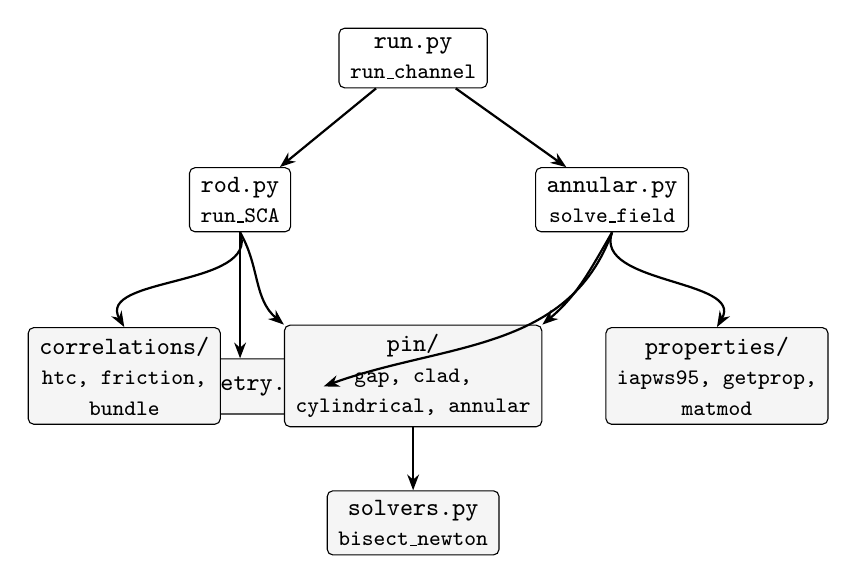
\begin{tikzpicture}[
  node distance=6mm,
  box/.style={draw, rounded corners=2pt, align=center, font=\small\ttfamily,
              minimum height=7mm, inner xsep=4pt},
  ext/.style={box, fill=codebg},
  arr/.style={-{Stealth[length=2mm]}, thick}
]
\node[box] (run) {run.py\\ \footnotesize run\_channel};
\node[box, below left=10mm and 6mm of run] (rod) {rod.py\\ \footnotesize run\_SCA};
\node[box, below right=10mm and 6mm of run] (ann) {annular.py\\ \footnotesize solve\_field};
\node[ext, below=16mm of rod] (geo) {geometry.py};
\node[ext, below=30mm of run] (pin) {pin/\\ \footnotesize gap, clad,\\ \footnotesize cylindrical, annular};
\node[ext, left=8mm of pin] (corr) {correlations/\\ \footnotesize htc, friction,\\ \footnotesize bundle};
\node[ext, right=8mm of pin] (prop) {properties/\\ \footnotesize iapws95, getprop,\\ \footnotesize matmod};
\node[ext, below=8mm of pin] (solv) {solvers.py\\ \footnotesize bisect\_newton};

\draw[arr] (run) -- (rod);
\draw[arr] (run) -- (ann);
\draw[arr] (rod) -- (geo);
\draw[arr] (ann.south) to[out=250,in=20] (geo.east);
\draw[arr] (rod.south) to[out=290,in=120] (corr.north);
\draw[arr] (ann.south) to[out=250,in=60] (prop.north);
\draw[arr] (rod.south) to[out=300,in=140] (pin.north west);
\draw[arr] (ann.south) to[out=240,in=40] (pin.north east);
\draw[arr] (pin) -- (solv);
\end{tikzpicture}
\end{center}

\code{lut.py} and \code{scw\_table.py} sit outside this graph entirely: nothing in the
module imports them. Part~\ref{part:legacy} explains what they are and why they are
still here.

\section{How to run one case}
\label{sec:howtorun}

Everything in Parts~IV--VII is an elaboration of this:

\begin{lstlisting}
from pinthac.sca.run import run_channel

out = run_channel(
    geometry={"type": "rod", "pitch": 0.0125, "rco": 0.0045,
              "tc": 0.00063, "delta": 5e-4, "kc": 24.0},
    conditions={"G": 1200.0, "pval": 25.0, "Tin": 573.15,
                "q0": 25e3, "L": 3.0, "N": 200},
    htc="swenson", friction="filonenko",
    bundle="presser", fuel_conductivity="klimenko",
)

print(out["convergence"]["ok"])              # True
print(max(out["result"]["T_fuel_max"]))      # 2523.72 K
print(out["result"]["dP"][-1] / 1000.0)      # 23.739 kPa
\end{lstlisting}

Four arguments select the physics by name; two dictionaries carry the geometry and the
operating conditions; one dictionary comes back with the axial solution and a
convergence report. Swapping \code{"type": "rod"} for \code{"type": "annular"} (with
that geometry's own keys) dispatches to a completely different solver through the same
call.

\newpage
%=======================================================================
\part{The physics, from scratch}
%=======================================================================

\noindent
This part assumes you can read an integral and nothing else. If you already know
reactor thermal hydraulics, skip to Part~\ref{part:data}.

\section{Notation and units}

PINTHAC is strict about units, and the naming is consistent across the whole library.
Every temperature, without exception, is in kelvin.

\begin{center}
\begin{tabular}{llll}
\toprule
Quantity & Symbol & Code & Unit \\
\midrule
Linear heat generation rate (LHGR) & $\qp$ & \code{qp}, \code{q0} & W/m \\
Surface heat flux                  & $\qpp$ & \code{qpp} & W/m$^2$ \\
Volumetric heat generation rate    & $\qppp$ & \code{q3}, \code{q\_ppp} & W/m$^3$ \\
Mass flux                          & $G$ & \code{G} & kg/m$^2$\,s \\
Mass flow rate                     & $\dot m$ & \code{mdot} & kg/s \\
Specific enthalpy                  & $h$ & \code{h} & J/kg (see warning below) \\
Hydraulic diameter                 & $D_h$ & \code{Dh}, \code{D} & m \\
Heat transfer coefficient          & $h_c$ & \code{htc} & W/m$^2$\,K \\
Bulk coolant temperature           & $T_m$ & \code{Tm}, \code{T\_i} & K \\
Wall temperature                   & $T_w$ & \code{Tw}, \code{Tco} & K \\
Conductivity integral              & $\Theta$ & \code{Theta} & W/m \\
Bundle correction factor           & $\psi$ & \code{psi} & --- \\
\bottomrule
\end{tabular}
\end{center}

\begin{quote}
\textbf{Enthalpy unit warning.} \code{rod.py}'s property table stores $h$ in
\textbf{J/kg}. \code{annular.py}'s \code{props\_at} returns $h$ in \textbf{J/kg} too,
but \code{\_T\_hp\_fast} takes $h$ in \textbf{kJ/kg} --- which is why
\code{solve\_field} calls it as \code{\_T\_hp\_fast(h\_i/1000.0, Pnom)}. This is the
single most likely place in the module to introduce a factor-of-1000 error.
\end{quote}

Pressures are \textbf{MPa} at every property interface and \textbf{Pa} inside the
momentum equation. \code{pval} and \code{Pnom} are MPa; the \code{dP} arrays are Pa.

\section{The axial energy balance}
\label{sec:axial}

Take a slice of channel of length $dz$. Coolant flows in at enthalpy $h_i$ and out at
$h_{i+1}$, and the rod deposits $\qp\,dz$ watts into it. Conservation of energy, with no
work and no axial conduction in the fluid:

\begin{equation}
\dot m \, (h_{i+1} - h_i) = \qp(z_i)\, dz
\qquad\Longrightarrow\qquad
h_{i+1} = h_i + \frac{\qp(z_i)\,dz}{\dot m}.
\label{eq:march}
\end{equation}

This is the whole axial march. Three things about it are worth stating explicitly
because they explain a great deal of the module's behaviour:

\begin{enumerate}
\item \textbf{It is written in enthalpy, not temperature.} Temperature is recovered
      afterwards from $T = T(h,p)$. You cannot write $\dot m\,c_p\,\Delta T$ instead,
      because supercritical water's $c_p$ is not remotely constant --- it spikes by a
      factor of ten at the pseudocritical temperature (Section~\ref{sec:pseudocritical}).
      Enthalpy is the conserved quantity; temperature is a derived one.
\item \textbf{No heat transfer coefficient appears anywhere in it.} The coolant's bulk
      temperature is set by how much energy went in, full stop. A wrong heat transfer
      correlation moves the \emph{wall} temperature, not the bulk. This is why
      \code{examples/monte\_carlo\_rod.py} finds exactly zero spread in outlet
      temperature when it perturbs the correlation by $\pm25\%$.
\item \textbf{It is strictly sequential.} Node $i+1$ needs node $i$. The axial loop
      cannot be vectorised away --- which is why \code{run\_SCA\_batch} parallelises
      over \emph{cases} instead, running $B$ independent rods through the same
      sequential axial loop at once (Section~\ref{sec:batch}).
\end{enumerate}

\subsection{The half-cell convention at the inlet}

Both solvers offset the first node. \code{rod.py}:

\begin{lstlisting}
Z = [-L/2 + dz + i*dz for i in range(n)]      # node centres
qp0 = q_p(-L/2 + dz/2)                        # power at the FIRST HALF-cell
h0  = hin + qp0*dz/mdot
\end{lstlisting}

and \code{annular.py}'s \code{march} does the same thing by a different route:

\begin{lstlisting}
def march(h0, q, mdot):
    e = np.empty(N)
    e[0]  = 0.5*q[0]        # only half a cell of power before the first node
    e[1:] = q[:-1]          # thereafter, the power UPSTREAM of this node
    return h0 + dz/mdot*np.cumsum(e)
\end{lstlisting}

The reason for \code{e[1:] = q[:-1]} is subtle and worth spelling out: node $i$'s
enthalpy reflects all the power deposited \emph{before} it. Writing \code{e[1:] = q[1:]}
would credit node $i$ with its own cell's power, which it has not yet passed through.
The shift is what makes the march a proper upwind integration rather than a
half-cell-too-hot one.

\section{The radial resistance chain}
\label{sec:chain}

Now the other half. At one axial node the coolant is at $T_m$ and the rod is producing
$\qp$ W/m. Work outward-in from the coolant to the fuel centre. Each step is a thermal
resistance, and the same $\qp$ flows through all of them.

\paragraph{Step 1: coolant to cladding outer surface (convection).}
\begin{equation}
T_{co} = T_m + \frac{\qp}{\pi d_o \, h_c}, \qquad d_o = 2 r_{co}.
\end{equation}
$h_c$ is the heat transfer coefficient from a correlation, and $\pi d_o$ is the wetted
perimeter, so $\qp/(\pi d_o)$ is the surface heat flux $\qpp$. This is Newton's law of
cooling, $\qpp = h_c\,(T_w - T_m)$, rearranged.

\paragraph{Step 2: through the cladding (conduction in a tube).}
\begin{equation}
T_{ci} = T_{co} + \frac{\qp}{2\pi k_c}\ln\!\left(\frac{r_{co}}{r_{ci}}\right).
\end{equation}
This is the exact steady solution of $\nabla^2 T = 0$ in an annulus with no internal
generation. The logarithm is the cylindrical analogue of the flat-plate $L/k$.

\paragraph{Step 3: across the gas gap (conduction {\bf and} radiation in parallel).}
The manufacturing gap between fuel and cladding is a few tens of microns of helium. Two
mechanisms cross it at once, so their conductances add:
\begin{equation}
h_{gap} = \underbrace{\frac{k_{gas}(\bar T)}{\delta}}_{\text{conduction}}
        + \underbrace{\frac{\sigma\,(T_{fo}^4 - T_{ci}^4)}{T_{fo} - T_{ci}}}_{\text{radiation, linearised}},
\qquad
T_{fo} = T_{ci} + \frac{\qp}{\pi (r_{ci}+r_{fo})\,h_{gap}}.
\label{eq:gap}
\end{equation}
The radiation term is written as an equivalent \emph{coefficient} by dividing the
Stefan--Boltzmann flux by the temperature difference it is driven by, so it can be added
to the conduction coefficient. Note that $h_{gap}$ depends on $T_{fo}$, which is what we
are solving for --- Equation~\eqref{eq:gap} is implicit, and the code root-finds it
(Section~\ref{sec:gap}).

The gas conductivity uses the Von Ubisch correlation $k_{gas} = 15.8\times10^{-4}\,
\bar T^{0.79}$ with $\bar T = (T_{fo}+T_{ci})/2$. \emph{The sign of that exponent was
wrong in the pre-cleanup code} --- it read $T^{-0.79}$, which puts $k_{gas}$ at
$10^{-5}$ instead of $0.25$~W/m\,K at 600~K, four orders of magnitude low. Gap
conduction effectively vanished and radiation carried the whole flux. Fixing it moved
peak fuel temperatures by $-430$ to $-510$~K. The comment at \code{rod.py:143} records
this.

\paragraph{Step 4: through the fuel to the centreline.}
This is the only step that is not a simple series resistance, because heat is being
\emph{generated} throughout the fuel rather than passing through it.
Section~\ref{sec:kirchhoff} handles it.

\section{Why the supercritical wall-temperature solve is implicit}
\label{sec:pseudocritical}

This is the single most important idea in the module. Everything awkward about both
solvers traces back to it.

Above the critical pressure (22.064~MPa for water) there is no boiling and no phase
boundary --- but there is still a sharp transition. At a fixed supercritical pressure,
as temperature rises through the \emph{pseudocritical} temperature $T_{pc}$ (about
658~K at 25~MPa), the fluid goes from liquid-like to gas-like over a span of a few tens
of kelvin. Across that span:

\begin{itemize}
\item density falls by a factor of roughly 5,
\item specific heat $c_p$ spikes to a sharp peak and falls again,
\item viscosity and thermal conductivity both drop steeply.
\end{itemize}

An ordinary heat transfer correlation like Dittus--Boelter evaluates all its properties
at the \emph{bulk} temperature. That is fine when properties barely change over the
film. Here they change enormously over the film, so a supercritical correlation
evaluates its properties at the \emph{wall} instead. Swenson's correlation is

\begin{equation}
\mathrm{Nu} = 0.00459\;\mathrm{Re}_w^{0.923}\;\mathrm{Pr}_w^{0.613}
             \left(\frac{\bar c_p}{c_{p,w}}\right)^{0.613}
             \left(\frac{\rho_w}{\rho_b}\right)^{0.231},
\qquad
h_c = \frac{\mathrm{Nu}\,k_w}{D_h},
\label{eq:swenson}
\end{equation}

where the subscript $w$ means ``evaluated at the wall temperature'' and
$\bar c_p = (h_w - h_b)/(T_w - T_b)$ is an integral-averaged specific heat across the
film.

Now look at what that does to the chain in Section~\ref{sec:chain}. Step~1 says
$T_w = T_m + \qpp/h_c$. But Equation~\eqref{eq:swenson} says $h_c$ is a function of
$T_w$. So:

\begin{equation}
\boxed{\;\text{solve}\quad F(T_w) \equiv (T_w - T_m) - \frac{\qpp}{\psi\,h_c(T_w)} = 0\;}
\label{eq:implicit}
\end{equation}

That is a genuine nonlinear scalar root-find, once per axial node, and it is why both
solvers carry a root-finder. It is also why the module distinguishes two classes of
correlation throughout:

\begin{center}
\begin{tabular}{lp{9.2cm}}
\toprule
\textbf{Implicit} & The correlation needs $T_w$ in its own formula. Requires solving
Equation~\eqref{eq:implicit}. In code: the \code{\_HTC\_DISPATCH} dict.
\newline \code{swenson}, \code{chen\_scw} \\
\midrule
\textbf{Explicit} & The correlation uses bulk properties only. Evaluate once, done. In
code: the \code{\_EXPLICIT\_HTC} dict.
\newline \code{dittus}, \code{petukhov}, \code{gnielinski}, \code{lyon}, \code{seban},
\code{mikityuk}, \code{lead\_shen} \\
\bottomrule
\end{tabular}
\end{center}

Both dicts appear, with identical structure, in \code{rod.py} (lines 254 and 268) and
\code{annular.py} (lines 238 and 248). \emph{Whether a correlation is implicit is a
property of the correlation, not of the solver} --- which is why the tables live next to
the solvers that dispatch on them rather than in \code{run.py}.

\subsection{Why $\psi$ is inside the residual}

Look carefully at Equation~\eqref{eq:implicit}: the bundle correction factor $\psi$ sits
\emph{inside} the residual, multiplying $h_c$, rather than being applied to the
converged answer afterwards. This matters. $\psi h_c$ is the coefficient that actually
sets the wall temperature, so the $T_w$ that satisfies the flux balance is the one found
with $\psi$ already in place. Solving without it and scaling afterwards gives a
different $T_w$, and therefore different wall-evaluated properties, and therefore a
different $h_c$. \code{rod.py:341} is the line that gets this right.

\section{The Kirchhoff transform}
\label{sec:kirchhoff}

The last step of the radial chain is conduction through fuel that is generating heat.
For a solid pellet with \emph{constant} conductivity $k_f$ the answer is the textbook
parabola,
\begin{equation}
T(0) - T(r_{fo}) = \frac{\qp}{4\pi k_f}.
\end{equation}
But UO$_2$'s conductivity is strongly temperature-dependent --- it falls by roughly
half between 800~K and 1800~K --- and a hot pin spans exactly that range. Using a
constant $k_f$ misplaces the centreline temperature badly.

The fix is a change of variable that makes the problem linear again. Define the
\textbf{conductivity integral}, also called the Kirchhoff transform:
\begin{equation}
\Theta(T) \;=\; \int_{T_{ref}}^{T} k_f(T')\,dT' \qquad [\mathrm{W/m}].
\label{eq:theta}
\end{equation}

Then $\nabla\Theta = k_f \nabla T$, so Fourier's law $\vec q = -k_f \nabla T$ becomes
simply $\vec q = -\nabla\Theta$, and the nonlinear conduction equation becomes a
\emph{linear} equation in $\Theta$. Solve it for $\Theta$, then invert
Equation~\eqref{eq:theta} once at the end to get the temperature.

$\Theta$ is strictly increasing, because $d\Theta/dT = k_f(T) > 0$ for any physical
conductivity. So the inversion has exactly one root and bisection cannot land on the
wrong branch --- a fact the solver relies on.

\subsection{Solid pellet: one inversion at the end}

For a solid pellet the linear solution in $\Theta$ is
\begin{equation}
\Theta(r) = \Theta_{fo} + \frac{\qppp}{4}\left(r_{fo}^2 - r^2\right),
\end{equation}
so the centreline value $\Theta(0) = \Theta_{fo} + \qppp r_{fo}^2/4$ is known
immediately, and a single root-find recovers $T(0)$. This is
\code{pin/cylindrical.py::Cyl\_T}, which \code{rod.py} calls at every node.

\subsection{Annular pellet: no inversion at all}
\label{sec:fluxsplit}

For an annulus the general solution carries two integration constants:
\begin{equation}
\Theta(r) \;=\; -\frac{\qppp}{4}r^2 + C_1 \ln r + C_2.
\label{eq:anngen}
\end{equation}

Given the $\Theta$ values at both fuel surfaces --- call them $\Theta_i$ at $r_i$ and
$\Theta_o$ at $r_o$ --- this is two linear equations in two unknowns, solved in closed
form by Cramer's rule:
\begin{align}
\alpha_i &= \Theta_i + \tfrac{\qppp}{4}r_i^2, &
\alpha_o &= \Theta_o + \tfrac{\qppp}{4}r_o^2, \\[2pt]
C_1 &= \frac{\alpha_i - \alpha_o}{\ln r_i - \ln r_o}, &
C_2 &= \frac{\ln r_i\,\alpha_o - \ln r_o\,\alpha_i}{\ln r_i - \ln r_o}.
\end{align}

The heat flux then follows by differentiating Equation~\eqref{eq:anngen}:
\begin{equation}
\qpp(r) = -\frac{d\Theta}{dr} = \frac{\qppp}{2}r - \frac{C_1}{r}.
\label{eq:annqpp}
\end{equation}

And \emph{that} is the power split. Evaluating Equation~\eqref{eq:annqpp} at $r_o$ gives
the outward flux, at $r_i$ the inward one:
\begin{lstlisting}
C1, C2 = ht.Ann_HT(ri, ro, q3, Theta_i, Theta_o)
q_i = -ht.Ann_qpp(ri, q3, C1) * Per_fuel_i     # note the minus
q_o =  ht.Ann_qpp(ro, q3, C1) * Per_fuel_o
\end{lstlisting}

Two things deserve emphasis.

\paragraph{The minus sign at the inner surface is deliberate and documented.}
Equation~\eqref{eq:annqpp} is written in the signed $+r$ Fourier convention: positive
means ``flowing toward larger $r$''. At the outer surface that is the physically outward
direction. At the inner surface it is not --- flow into the inner coolant is toward
\emph{smaller} $r$ --- so the physical flux there is the negative. The reference
derivation PDF states the inner-surface relation without this minus, and following it
literally converges to a state with the inner wall \emph{colder} than the inner coolant
and a badly violated energy balance. The departure is recorded in
\code{docs/DECISIONS.md} (closing Q18) and tested.

\paragraph{$\Theta$ is only ever evaluated forwards.} $\Theta_i$ and $\Theta_o$ come
from surface temperatures the closure loop already has, so
Equation~\eqref{eq:theta} is evaluated in the easy direction. Unlike the solid-pellet
case, the annular scheme never inverts $\Theta$ at all. That is the entire point of
formulating it this way, and it is why \code{Ann\_Theta} can return a cheap
one-directional spline interpolant.

\paragraph{The energy balance is exact at every iterate.} Adding the two fluxes:
\begin{equation}
q_i + q_o = \qppp\,\pi\,(r_o^2 - r_i^2)
\end{equation}
holds identically --- the $C_1$ terms cancel algebraically, not approximately. It holds
on the very first Picard guess, not just at convergence, which is what makes it a useful
\emph{invariant} to test rather than a convergence check. \code{tests/test\_annular.py}
measures it at $4.8\times10^{-16}$ relative.

\section{Pressure drop}
\label{sec:dp}

Both solvers compute the same three-term single-phase momentum balance, cell by cell,
after the temperature field is known. Writing $v = 1/\rho$ for specific volume:

\begin{equation}
\Delta P_{cell} =
\underbrace{f\,\frac{dz}{D_h}\,\frac{G^2 \bar v}{2}}_{\text{friction}}
+ \underbrace{\frac{g\,dz}{\bar v}}_{\text{gravity}}
+ \underbrace{G^2\,(v_i - v_{i-1})}_{\text{acceleration}},
\qquad \bar v = \tfrac{1}{2}(v_{i-1} + v_i),
\end{equation}

and the reported \code{dP} is the running cumulative sum, with \code{dP[0] = 0} because
no drop has yet been accumulated across the inlet half-cell.

The acceleration term is not negligible here. Supercritical water expands by a factor of
several through the pseudocritical transition, so $G^2\Delta v$ is a real contribution
in a channel that crosses $T_{pc}$ --- unlike a subcooled PWR channel where it is
usually dropped.

$f$ comes from a friction correlation; the default is Filonenko. Note that
\code{annular.py} uses Filonenko on \emph{both} channels, including the outer rod-bundle
one, even though Wu is the rod-bundle-fitted alternative. The reason is a hard limit:
Wu's validated range stops at $G = 1000$~kg/m$^2$\,s, which realistic cases exceed.

\newpage
%=======================================================================
\part{The data that moves between the pieces}
\label{part:data}
%=======================================================================

\noindent
Everything in this module is a plain dictionary. There are no classes with state, no
objects to construct, no configuration files. Five dictionary shapes account for the
entire module, and knowing them is most of knowing the code.

\section{The \code{geometry} dictionary}

Passed by the user to \code{run\_channel}. It must carry a \code{"type"} key naming the
geometry family; every other key depends on which family.

\subsection{Rod geometry}
Required keys, from \code{run.py:85} (\code{\_ROD\_GEOM\_KEYS}). All are required; a
missing one raises immediately with the full list.

\begin{center}
\begin{tabular}{llp{7.0cm}}
\toprule
Key & Unit & Meaning \\
\midrule
\code{pitch} & m & rod-to-rod spacing in the square lattice \\
\code{rco}   & m & cladding \emph{outer} radius --- the wetted surface \\
\code{tc}    & m & cladding wall thickness; $r_{ci} = r_{co} - t_c$ \\
\code{delta} & m & radial gas-gap width; $r_{fo} = r_{ci} - \delta$ \\
\code{kc}    & W/m\,K & cladding thermal conductivity, taken as constant \\
\bottomrule
\end{tabular}
\end{center}

Note the geometry is specified from the outside in. You give the cladding OD and
subtract thicknesses to reach the fuel, rather than giving a pellet radius and adding
outward.

\subsection{Annular geometry}
From \code{run.py:90} (\code{\_ANNULAR\_GEOM\_KEYS}). Again all required.

\begin{center}
\begin{tabular}{llp{7.2cm}}
\toprule
Key & Unit & Meaning \\
\midrule
\code{ri}      & m & fuel \emph{inner} radius (the bore side) \\
\code{ro}      & m & fuel \emph{outer} radius \\
\code{tci}     & m & inner cladding thickness \\
\code{tco}     & m & outer cladding thickness \\
\code{delta\_i} & m & inner gas-gap width \\
\code{delta\_o} & m & outer gas-gap width \\
\code{Pitch}   & m & lattice pitch (capital P --- the annular solver's own spelling) \\
\code{Gas}     & --- & gap fill gas name, defaulted to \code{"He"} if omitted \\
\bottomrule
\end{tabular}
\end{center}

Here the fuel surfaces are given directly and the cladding is built \emph{outward} from
them in both directions --- the opposite convention from the rod case. This asymmetry is
a genuine inconsistency in the module's input design, inherited from the two solvers'
separate histories; \code{run.py} papers over it but does not remove it.

\begin{quote}
\textbf{Historical note.} \code{annular.py} used to carry a module-level
\code{Inputs\_ann} dictionary --- a complete default case baked into the solver file.
It was removed. A solver is not an example, and a default geometry silently standing in
for one the caller forgot is how a run ends up reporting somebody else's pin. The
comment at \code{run.py:86--89} records this, and every annular key is now required with
no fallback.
\end{quote}

\section{The \code{conditions} dictionary}

\begin{center}
\begin{tabular}{lllp{5.6cm}}
\toprule
Key & Geometry & Unit & Meaning \\
\midrule
\code{G}      & rod & kg/m$^2$\,s & coolant mass flux \\
\code{pval}   & rod & MPa & system pressure, held fixed along the channel \\
\code{Tin}    & rod & K & coolant inlet temperature \\
\code{q0}     & both & W/m & \emph{peak} LHGR of the cosine shape \\
\code{L}      & both & m & heated length (rod default 3.0) \\
\code{N}      & both & --- & axial nodes (rod default 400, annular default 100) \\
\midrule
\code{Tin\_i} & annular & K & inner-channel inlet temperature \\
\code{Tin\_o} & annular & K & outer-channel inlet temperature \\
\code{Pnom}   & annular & MPa & system pressure \\
\code{mdot\_i} & annular & kg/s & inner-channel mass flow rate \\
\code{mdot\_o} & annular & kg/s & outer-channel mass flow rate \\
\bottomrule
\end{tabular}
\end{center}

The rod path specifies flow as a mass \emph{flux} $G$ and derives $\dot m = G A_{flow}$;
the annular path specifies mass flow \emph{rate} directly for each channel and derives
$G = \dot m / A_{flow}$. Same second inconsistency, same cause.

Both solvers default the axial power to a cosine shape,
\begin{equation}
\qp(z) = q_0 \cos\!\left(\frac{\pi z}{L}\right), \qquad z \in [-L/2,\, L/2],
\end{equation}
which is the classic chopped-cosine profile of an unreflected, uniformly enriched core.
\code{annular.solve\_field} accepts a \code{q\_p=} callable to override it;
\code{rod.run\_SCA\_batch} takes sampled values instead (Section~\ref{sec:batch}).

\section{The \code{Props} dictionary}
\label{sec:props}

The universal property-bundle convention, shared with \code{correlations/}. Every
correlation in the library takes one or two of these.

\begin{center}
\begin{tabular}{lll}
\toprule
Key & Unit & Quantity \\
\midrule
\code{rho} & kg/m$^3$ & density \\
\code{mu}  & Pa\,s & dynamic viscosity \\
\code{k}   & W/m\,K & thermal conductivity \\
\code{cp}  & J/kg\,K & isobaric specific heat \\
\code{h}   & J/kg & specific enthalpy \\
\bottomrule
\end{tabular}
\end{center}

Two conventions surround it. \code{Props\_b} means properties at the \emph{bulk}
temperature; \code{Props\_w} means at the \emph{wall}. Implicit correlations
(Section~\ref{sec:pseudocritical}) need both.

The three producers of \code{Props} in this module are worth contrasting directly,
because the difference is the whole subject of Section~\ref{sec:lutopportunity}:

\begin{center}
\begin{tabular}{lp{4.1cm}p{5.4cm}}
\toprule
Producer & Backed by & Used by \\
\midrule
\code{rod.\_props\_at} & 3000-point table, linear interpolation in $T$, on GPU & \code{rod.py} \\
\code{annular.props\_at} & \textbf{live IAPWS-95 call} & \code{annular.py} \\
\code{lut.Props\_TP} & 2-D $(T,P)$ table, SciPy interpolation & \code{lut.py} only \\
\bottomrule
\end{tabular}
\end{center}

\section{The result dictionaries}

\subsection{\code{rod.run\_SCA} returns}
\begin{center}
\begin{tabular}{llp{6.2cm}}
\toprule
Key & Type & Meaning \\
\midrule
\code{Z}          & list, length $n$ & axial node centres, m, from $-L/2$ \\
\code{T\_i}       & list of float & bulk coolant temperature, K \\
\code{qp}         & list of float & local LHGR, W/m \\
\code{T\_fuel\_max} & list of float & fuel centreline temperature, K \\
\code{dP}         & numpy array & cumulative pressure drop, Pa \\
\bottomrule
\end{tabular}
\end{center}

\subsection{\code{annular.solve\_field} returns}
Much richer, because the annular chain has twice as many surfaces and the outer loop has
convergence state worth reporting. All values are NumPy arrays of length $N$ except the
last three scalars.

\begin{center}
\begin{tabular}{llp{6.0cm}}
\toprule
Key & Unit & Meaning \\
\midrule
\code{z} & m & axial node centres \\
\code{h\_i}, \code{h\_o} & J/kg & inner/outer channel enthalpy \\
\code{Tm\_i}, \code{Tm\_o} & K & inner/outer bulk coolant temperature \\
\code{Tfo\_i}, \code{Tfo\_o} & K & fuel surface temperature, inner/outer side \\
\code{Tcldi\_ID}, \code{Tcldi\_OD} & K & inner cladding, both faces \\
\code{Tcldo\_ID}, \code{Tcldo\_OD} & K & outer cladding, both faces \\
\code{htc\_conv\_i}, \code{htc\_conv\_o} & W/m$^2$K & convective coefficients \\
\code{htc\_gap\_i}, \code{htc\_gap\_o} & W/m$^2$K & gap coefficients \\
\code{q\_i}, \code{q\_o} & W/m & the converged power split \\
\code{dP\_i}, \code{dP\_o} & Pa & cumulative pressure drop per channel \\
\code{outer\_converged} & bool & did the outer Picard loop meet \code{tol}? \\
\code{outer\_residual} & J/kg & final enthalpy residual \\
\code{outer\_iters\_used} & --- & iterations actually taken \\
\bottomrule
\end{tabular}
\end{center}

Note there is \emph{no} fuel centreline temperature in the annular output. The annular
scheme deliberately never inverts $\Theta$ (Section~\ref{sec:fluxsplit}), so it reports
fuel \emph{surface} temperatures only. Recovering the peak would need one extra
inversion, which is not currently done.

\subsection{\code{run\_channel} returns}
The outermost wrapper, from \code{run.py:309}:
\begin{center}
\begin{tabular}{lp{9.0cm}}
\toprule
Key & Meaning \\
\midrule
\code{result} & the underlying solver's own dict, verbatim \\
\code{geom\_type} & \code{"rod"} or \code{"annular"} \\
\code{requested} & the four correlation names as given \\
\code{convergence} & the report from \code{\_scan\_for\_nonfinite}, plus the annular
outer-loop fields \\
\code{notes} & list of strings; always empty today (see \S\ref{sec:notes}) \\
\bottomrule
\end{tabular}
\end{center}

\newpage
%=======================================================================
\part{\code{run.py} --- the driver}
%=======================================================================

\noindent
430 lines, four public functions, three private helpers. This is the only file most
users will ever call. Its job is: validate, translate, dispatch, report.

\section{The four selection tables}

Lines 50--81. Four plain dictionary literals mapping a name string to a function.

\begin{lstlisting}
HTC_MODELS = {
    "swenson":  htc.SCW.Swenson_dT,
    "chen_scw": htc.SCW.Chen_SCW_dT,
    "dittus":   htc.Water.Dittus,
    ...
}
FRICTION_MODELS = {"filonenko": fric.f_SCW.Filonenko, "wu": fric.f_SCW.Wu, ...}
BUNDLE_MODELS   = {"presser": bundle_mod.Bundle.Presser,
                   "weissman": bundle_mod.Bundle.Weissman}
FUEL_CONDUCTIVITY_MODELS = {
    "klimenko": (matmod.UO2.k_Klimenko, matmod.UO2.Theta_Klimenko),
    "nfi":      (matmod.UO2.k_NFI,      matmod.UO2.Theta_NFI),
}
\end{lstlisting}

The full name lists:

\begin{center}
\begin{tabular}{lp{9.4cm}}
\toprule
Category & Valid names \\
\midrule
\code{htc} & \code{swenson}, \code{chen\_scw}, \code{dittus}, \code{gnielinski},
\code{petukhov}, \code{lyon}, \code{seban}, \code{mikityuk}, \code{lead\_shen}; plus
\code{chen\_h2o}, \code{bjorge}, \code{schrock\_grossman}, which are recognised but
raise (\S\ref{sec:twophase}) \\
\code{friction} & \code{filonenko}, \code{wu}, \code{blasius}, \code{mcadams},
\code{colebrook} \\
\code{bundle} & \code{presser}, \code{weissman}, or \code{None} for no correction \\
\code{fuel\_conductivity} & \code{klimenko}, \code{nfi} \\
\bottomrule
\end{tabular}
\end{center}

Two design notes.

\paragraph{Fuel conductivity is a \emph{pair}.} $(k_f, \Theta)$ travel together because
\code{Cyl\_T} needs both --- $\Theta$ to state the problem and $k_f$ as its analytic
derivative for the Newton polish. The two are related by
Equation~\eqref{eq:theta}: \code{k\_Klimenko} is exactly $d\Theta_{\text{Klimenko}}/dT$.
That identity was established during the Phase~3 conductivity-integral fix and is what
makes supplying \code{k\_func} to \code{Cyl\_T} legitimate rather than an approximation.

\paragraph{There is no registry.} No plugin system, no entry points, no
auto-discovery, no configuration language. A dict literal and a lookup. This is a
deliberate constraint --- the alternative mechanisms were all forbidden by name in the
phase brief --- and it means a reader can see the entire set of available physics by
reading 30 lines.

\section{\code{\_select(name, table, category)}}
Line 95. Eleven lines, and the only place a correlation name is ever resolved.

\begin{lstlisting}
def _select(name, table, category):
    if name is None:
        return None                      # only 'bundle' uses this: no correction
    if name not in table:
        raise ValueError(
            f"{category}: unknown model {name!r} -- valid options are {sorted(table)}")
    return table[name]
\end{lstlisting}

It fails immediately and prints the valid options. There is no partial matching, no
case-folding, no fallback to a default on a miss. A typo is an error at the top of the
run, not a silently-different physics model discovered three figures later.

\code{None} passes through untouched, which is how \code{bundle=None} means ``apply no
rod-bundle correction, $\psi = 1$''.

\section{\code{\_rod\_inputs} and \code{\_annular\_inputs}}
Lines 155 and 180. These are the translators: user-facing dictionaries in, each solver's
own private input format out.

\code{\_rod\_inputs} splits its output in two, because \code{rod.run\_SCA} takes geometry
as a dict but conditions as keyword arguments:
\begin{lstlisting}
inputs = {k: geometry[k] for k in _ROD_GEOM_KEYS}
inputs["G"] = conditions["G"]                  # G rides in the geometry dict
run_kwargs = dict(pval=..., Tscw_in=..., q0=..., L=..., n=...)
\end{lstlisting}
Note \code{G} being folded into \code{inputs} rather than \code{run\_kwargs} --- that is
\code{rod\_node}'s expectation, not a mistake.

\code{\_annular\_inputs} instead \emph{merges} geometry and conditions into one flat
dict, because that is what \code{solve\_field} takes:
\begin{lstlisting}
merged = dict(geometry); merged.update(conditions)
missing = [k for k in _ANNULAR_GEOM_KEYS + _ANNULAR_COND_KEYS if k not in merged]
if missing: raise ValueError(...)
merged.setdefault("N", 100)
merged.setdefault("Gas", "He")
\end{lstlisting}
Only \code{N} and \code{Gas} get defaults --- a discretisation choice and a fill-gas
choice. No \emph{physical} quantity is ever defaulted.

Both raise a \code{ValueError} naming exactly which keys are missing and listing the
full required set. This exists so a mistake surfaces as a sentence rather than as a
\code{KeyError} thrown from three frames deep inside a solver.

\section{\code{run\_channel(...)} --- the main entry point}
Line 199. The function everything else in this document exists to explain. Its body is
short; read it as six phases.

\paragraph{Phase 1 --- validate the geometry type.}
\begin{lstlisting}
geom_type = geometry.get("type")
if geom_type not in ("rod", "annular"):
    raise ValueError(...)
\end{lstlisting}

\paragraph{Phase 2 --- resolve every correlation name.}
\begin{lstlisting}
_select(htc, HTC_MODELS, "htc")          # validated, return deliberately discarded
friction_func = _select(friction, FRICTION_MODELS, "friction")
bundle_func   = _select(bundle,   BUNDLE_MODELS,   "bundle")
k_func, Theta_func = _select(fuel_conductivity, FUEL_CONDUCTIVITY_MODELS, ...)
\end{lstlisting}

The first line is the odd one. Its return value is thrown away --- called purely so an
unknown \code{htc} name fails here, with the valid list, rather than deeper inside a
solver. The \emph{name} is what gets passed down (\code{htc\_name=htc}), not the
function, because the solvers dispatch on the name themselves to decide implicit versus
explicit (Section~\ref{sec:pseudocritical}). The other three categories have no such
distinction, so their resolved functions are passed directly.

\paragraph{Phase 3 --- reject two-phase selections.}
\label{sec:twophase}
\begin{lstlisting}
if htc in _TWO_PHASE_HTC:
    raise NotImplementedError(...)
\end{lstlisting}
Chen, Bjorge and Schrock--Grossman are real, implemented, tested correlations in
\code{correlations/htc.py}. But neither solver has any boiling machinery --- no
onset-of-nucleate-boiling criterion, no quality or void-fraction tracking, no
subcooled-boiling bookkeeping. Both march a single-phase enthalpy balance and nothing
else. Selecting one therefore raises rather than silently marching a boiling channel
that does not exist. This is a deliberate, documented gap, not an oversight.

\paragraph{Phase 4 --- dispatch.}
\begin{lstlisting}
if geom_type == "rod":
    inputs, run_kwargs = _rod_inputs(geom_only, conditions)
    run_kwargs.update(solver_kwargs)
    result = rod.run_SCA(inputs, htc_name=htc, friction_func=friction_func,
                         bundle_func=bundle_func, k_func=k_func,
                         Theta_func=Theta_func, **run_kwargs)
else:
    inp = _annular_inputs(geom_only, conditions)
    result = annular.solve_field(inp, htc_name=htc, friction_func=friction_func,
                                 bundle_func=bundle_func, k_func=k_func,
                                 **solver_kwargs)
\end{lstlisting}

Note the asymmetry in the last argument: the rod path passes both \code{k\_func} and
\code{Theta\_func}; the annular path passes \code{k\_func} only. That is correct. The
annular solver builds its own $\Theta$ from $k$ via \code{Ann\_Theta} --- a numerically
integrated spline --- because it needs a callable it can evaluate at arbitrary
temperatures cheaply and only ever forwards. The rod solver needs the analytic
$\Theta$ because it must \emph{invert} it, and it wants the exact $k$ as the derivative
for the Newton polish.

\code{**solver\_kwargs} is the escape hatch: anything the caller passes that
\code{run\_channel} does not recognise goes straight through to the dispatched solver.
That is how \code{tol=}, \code{outer\_iter=}, \code{progress=}, \code{scw\_table=} and
\code{device=} reach their destinations without \code{run\_channel} having to name every
knob.

\paragraph{Phase 5 --- build the convergence report.}
\begin{lstlisting}
convergence = _scan_for_nonfinite(result, "Z", ("T_i", "T_fuel_max", "dP"))
\end{lstlisting}
and for the annular case, additionally, the outer-loop state:
\begin{lstlisting}
convergence["outer_converged"] = bool(result["outer_converged"])
convergence["outer_residual"]  = result["outer_residual"]
convergence["outer_iters_used"] = result["outer_iters_used"]
if not result["outer_converged"]:
    convergence["ok"] = False
    convergence["message"] += " -- also, the outer enthalpy Picard loop did not ..."
\end{lstlisting}

\paragraph{Phase 6 --- return.} The five-key dict of Part~\ref{part:data}.

\section{\code{\_scan\_for\_nonfinite}}
Line 121. The reason a bad case produces a sentence instead of a silent NaN.

\begin{lstlisting}
z = np.asarray(result[z_key], dtype=float)
for field in fields:
    values = np.asarray(result[field], dtype=float)
    bad = np.flatnonzero(~np.isfinite(values))
    if bad.size:
        i = int(bad[0])
        return dict(ok=False, node=i, z=float(z[i]), field=field,
                    message=f"{field} is non-finite ... at node {i} (z = {z[i]:.4f} m)")
return dict(ok=True, ..., message="every tracked field is finite at every axial node")
\end{lstlisting}

The motivation is worth stating plainly. Neither solver raises on a physically
nonsensical case. \code{bisect\_newton} runs a fixed iteration count and returns
whatever it has; a bracket that never straddled the root just yields garbage. A diverging
Picard iterate comes out as \code{inf}. Both propagate quietly into the output arrays.
This function turns that into a \emph{located} failure: which field, which node, which
axial position. It reports the first occurrence only, and says so.

The fields scanned differ by geometry: \code{("T\_i", "T\_fuel\_max", "dP")} for the rod,
\code{("Tm\_i", "Tm\_o", "Tfo\_i", "Tfo\_o", "q\_i", "q\_o")} for the annulus.

\section{\code{run\_batch(cases)}}
Line 313. A loop over \code{run\_channel} with one significant addition: error isolation.

\begin{lstlisting}
for i, case in enumerate(cases):
    kwargs = {k: v for k, v in case.items() if k not in ("geometry", "conditions")}
    try:
        out = run_channel(case["geometry"], case["conditions"], **kwargs)
        out["case_index"] = i
    except (ValueError, NotImplementedError, KeyError) as exc:
        out = dict(case_index=i, error=str(exc))
    results.append(out)
\end{lstlisting}

One bad case --- a typo'd correlation name, a geometry missing a key --- is recorded and
skipped rather than killing the other 9,999 cases in a sweep. The returned list is
always the same length and order as the input, so results line up with cases
positionally; each entry either has \code{"result"} or has \code{"error"}.

This is the module's only \code{try}/\code{except}. \code{CLAUDE.md} section~2 forbids
exceptions as control flow, and this is the documented exception to that rule: it catches
an \emph{actual} exception at a batch boundary to isolate one case's failure, which is
precisely what \code{run\_channel} raises to signal.

Because the correlation keys are per-case, ``one geometry across several correlations''
is just the same geometry repeated with different \code{htc=} values --- which is how the
comparison figures are generated.

\section{\code{read\_cases\_csv(path, geom\_type)}}
Line 356. A spreadsheet reader, in the spirit of the original project's Excel-driven
input.

Each row becomes one case dict. Columns named \code{htc}, \code{friction},
\code{bundle} or \code{fuel\_conductivity} become that row's correlation override;
every other column becomes a geometry or condition value, sorted into the right
dictionary by the same key lists \code{\_rod\_inputs}/\code{\_annular\_inputs} use.

Two limitations, both deliberate:
\begin{itemize}
\item \textbf{CSV only, not XLSX.} \code{openpyxl} is not installed and adding a
      dependency was not approved. Export the sheet to \code{.csv} first.
\item \textbf{One geometry family per file.} \code{geom\_type} is an argument, not a
      per-row column. Mixing rod and annular cases in one file is not supported.
\end{itemize}

For the annular branch the reader puts \emph{everything} into \code{geometry} and leaves
\code{conditions} empty --- which works only because \code{\_annular\_inputs} merges the
two dicts anyway before checking for missing keys.

\section{The \code{notes} channel}
\label{sec:notes}
\code{run\_channel} always returns \code{notes: []}. It is an always-present,
normally-empty channel for anything a caller should know about a run that is not an
error.

It exists because of a real historical situation. In the first version of this file
(commit \code{57ca0a1}) \code{rod.py} and \code{annular.py} had their per-node physics
hardcoded --- Swenson, Filonenko, Presser, Klimenko, and nothing else --- so
\code{run\_channel} could accept a correlation name it had no way to honour. A helper
called \code{\_unhonored\_notes} compared what was requested against what the solver was
actually fixed to, and reported the difference in this list, so that a run at least told
you which of your selections had been ignored.

The \code{sca} rework (commit \code{cc2991d}) fixed the underlying problem rather than
the reporting: every selection now genuinely reaches the solver, \code{\_unhonored\_notes}
is gone, and nothing writes to \code{notes} any more. It is kept in the return shape so
that a future category which cannot be fully honoured has somewhere to say so, rather
than regressing to silence.

\newpage
%=======================================================================
\part{\code{geometry.py} --- the shared unit cells}
%=======================================================================

\noindent
87 lines, two functions, no state, no physics beyond arithmetic. It exists because the
same two formulas were previously written by hand in three places.

\section{\code{square\_pitch\_cell(pitch, R)}}

The coolant region around one rod in a square lattice: the $p \times p$ square minus the
circle of radius $R$.
\begin{align}
A_{flow} &= p^2 - \pi R^2 & &[\mathrm{m^2}] \\
P_{wet}  &= 2\pi R        & &[\mathrm{m}] \\
D_h      &= \frac{4 A_{flow}}{P_{wet}} & &[\mathrm{m}]
\end{align}

The hydraulic diameter $D_h = 4A/P$ is the standard device for reusing round-tube
correlations in a non-round channel: it is defined so that a circular tube reproduces its
own diameter, and every friction and heat-transfer correlation in the library takes it
where a tube diameter would otherwise go.

Note the wetted perimeter counts \emph{only} the rod surface, not the four notional
square boundaries. Those are symmetry planes between adjacent rods --- no shear, no heat
flux --- so they are not wetted walls.

Used by: \code{rod.py}'s single coolant channel, and \code{annular.py}'s outer channel.

\section{\code{circular\_channel(R)}}
\begin{equation}
A_{flow} = \pi R^2, \qquad P_{wet} = 2\pi R, \qquad D_h = \frac{4A_{flow}}{P_{wet}} = 2R.
\end{equation}
The hydraulic diameter of a circular channel is trivially its own diameter. Writing it
out in the same $A/P/D_h$ shape anyway keeps both channel types identical at the call
site, so \code{annular.geometry} reads the same for its bore and its lattice cell.

Used by: \code{annular.py}'s inner channel.

\newpage
%=======================================================================
\part{\code{rod.py} --- the solid-rod solver}
%=======================================================================

\noindent
555 lines. Torch-based throughout, so it runs on GPU and can solve a whole batch of
independent rods at once. Read it in execution order: build the property table, march
axially, and at each node walk the radial chain inward.

\section{\code{build\_scw\_table(p, Tmin, Tmax, n, device)}}
\label{sec:scwtable}
Line 79. Called once per run, before anything else.

\begin{lstlisting}
T   = np.linspace(Tmin, Tmax, n)         # 290-1000 K, n = 3000
rho = IAPWS95.rho_Tp(T, p)
d   = IAPWS95.helmholtz(rho, T)
table = {'T': T, 'rho': rho, 'mu': IAPWS95.mu(d), 'k': IAPWS95.lam(d),
         'h': IAPWS95.h(d), 'cp': IAPWS95.cp(d)}
return {k: torch.as_tensor(v, dtype=DTYPE, device=device) for k, v in table.items()}
\end{lstlisting}

This is the module's single most consequential performance decision. It evaluates the
full IAPWS-95 equation of state \textbf{once}, as a single batched call over 3000 state
points, and every property lookup for the rest of the run is a table interpolation. A
400-node channel with three root-finds per node would otherwise reach the equation of
state tens of thousands of times, in small batches that amortise none of its fixed
per-call overhead.

Three details:

\paragraph{It is a 1-D table in $T$ only.} Pressure is fixed at \code{pval} for the
whole channel. The pressure drop is computed, reported, and then \emph{not} fed back into
the property lookups. This is a real approximation --- a tolerable one, since a 24~kPa
drop against a 25~MPa system pressure is one part in a thousand, and supercritical water
properties are far more sensitive to $T$ than to $p$ over that range. \code{lut.py}
(Part~\ref{part:legacy}) is the module's one example of doing it the other way.

\paragraph{The table is built through NumPy, deliberately.} The comment at lines 65--78
explains: \code{IAPWS\_97}'s viscosity and conductivity constants are plain CPU tensors
with no \code{device=} set, so a genuinely CUDA-resident $T$ hits a ``tensors on cuda:0
and cpu'' mismatch that the NumPy path never triggers. That is a pre-existing bug in the
shared property library. The table is therefore built on CPU and \emph{then} moved onto
the target device as torch tensors, so the actually-GPU-capable part of the module ---
the lookups and the root-finder --- still runs on GPU.

\paragraph{\code{h} is stored in J/kg and \code{cp} in J/kg\,K.} The SI defaults.

\section{\code{make\_Property(df)}}
Line 94. Returns a \emph{closure} that interpolates the table.

\begin{lstlisting}
def Property(Prop, prop):
    x, y = df[Prop[0]], df[prop]
    xq   = torch.as_tensor(Prop[1], dtype=DTYPE, device=x.device)
    xq_c = xq.clamp(x[0], x[-1])
    idx  = torch.searchsorted(x, xq_c).clamp(1, x.shape[0] - 1)
    x0, x1 = x[idx-1], x[idx]
    y0, y1 = y[idx-1], y[idx]
    w = (xq_c - x0) / (x1 - x0)
    return y0 + w*(y1 - y0)
\end{lstlisting}

The calling convention is unusual and worth decoding. \code{Property(['T', 600.0],
'rho')} means ``interpolate \code{rho} against the \code{T} column, at $T = 600$~K''. The
first argument is a \emph{(which column to look up in, at what value)} pair; the second
names the column you want out.

This lets the same function be used in both directions, which the axial march needs:
\begin{lstlisting}
h = Property(['T', T], 'h')     # T -> h, used once at the inlet
T = Property(['h', h], 'T')     # h -> T, used at EVERY axial node
\end{lstlisting}
The reverse lookup works because $h$ is monotone in $T$ away from the two-phase dome,
so the \code{h} column is sorted ascending and \code{searchsorted} is valid on it.
\textbf{This is what replaces a root-find for the $h \to T$ inversion} --- and it is the
single biggest reason the rod solver is fast where the annular solver is not
(\S\ref{sec:lutopportunity}).

Out-of-range queries \emph{clamp} to the table edge rather than extrapolating. Silent, so
a case that drifts outside 290--1000~K produces a plausible-looking edge value rather
than an obvious failure.

\code{torch.searchsorted} is the whole reason this is a torch table rather than a
\code{scipy.interpolate.interp1d}: it is batched and device-resident, so a lookup on a
$(B,)$ tensor of temperatures is one kernel launch.

\section{\code{run\_SCA(...)} --- the axial march}
Line 417. The rod solver's main routine.

\begin{lstlisting}
if scw_table is None:
    scw_table = build_scw_table(pval, device=device)
Property = make_Property(scw_table)

dz = L/n
Z  = [-L/2 + dz + i*dz for i in range(n)]
q_p = lambda z: q0*math.cos(math.pi*z/L)

cell = geometry.square_pitch_cell(inputs['pitch'], inputs['rco'])
Dh   = cell['Dh']
mdot = inputs['G'] * cell['A_flow']
\end{lstlisting}

Then the inlet half-cell, then the loop:

\begin{lstlisting}
hin  = Property(['T', Tin_t], 'h')
qp0  = q_p(-L/2 + dz/2)
_, Tmax0 = node(Tin_t, qp0_t)              # radial solve at the INLET temperature
h0   = hin + qp0_t*dz/mdot
T0   = Property(['h', h0], 'T')

for i in range(1, n):
    qp_local = q_p(Z[i] - dz/2)
    _, Tmax  = node(T_i[i-1], qp_t)        # radial solve at the PREVIOUS node's T
    h_scw    = h_i[i-1] + qp_t*dz/mdot     # axial step, Eq. (2)
    T_scw    = Property(['h', h_scw], 'T')
\end{lstlisting}

The structure is exactly Section~\ref{sec:axial} plus Section~\ref{sec:chain}: one
enthalpy step and one independent radial solve per node. Note the radial solve uses
\code{T\_i[i-1]}, the \emph{upstream} bulk temperature, consistent with the upwind
enthalpy march.

Finally, after the whole temperature field exists:
\begin{lstlisting}
dP = pressure_drop(np.array(T_i_list), inputs['G'], Dh, scw_table, friction_func, dz)
\end{lstlisting}
Pressure drop is a post-pass, not part of the march, because nothing in the march depends
on it (the property table is at fixed $p$).

The returned lists are cast to plain Python floats, which means \textbf{the scalar path
is not differentiable}. Gradients survive only through \code{run\_SCA\_batch}, which
keeps everything as tensors.

\section{\code{rod\_node(...)} --- the radial chain}
Line 346. Called once per axial node. Thirty lines that implement all of
Section~\ref{sec:chain}.

\begin{lstlisting}
rci = rco - tc
rfo = rci - delta
d_o = 2*rco
A_fuel = math.pi*rfo**2
q_ppp  = qp_val/A_fuel                     # W/m^3

cell = geometry.square_pitch_cell(pitch, rco)
Dh   = cell['Dh']
psi  = bundle_func(pitch, d_o) if bundle_func is not None else 1.0

htc_conv = htc_scw(Property, Tm, qp_val, p, G, Dh, psi, htc_name=htc_name, pitch=pitch)
Tco  = Tm  + qp_val/(math.pi*d_o*htc_conv)                  # convection
Tci  = Tco + qp_val/(2*math.pi*kc)*_log(rco/rci)            # clad conduction
Tfo  = gap(qp_val, delta, Tci, rci, rfo)                    # gap, implicit

Theta_fo = Theta_func(Tfo)
Tmax = Cyl_T(0.0, rfo, q_ppp, Theta_fo, Theta_func, k_func=k_func,
             T_lo=1.0, T_hi=6000.0)                         # fuel, Kirchhoff
return Tco, Tmax
\end{lstlisting}

Line for line against Section~\ref{sec:chain}: Step~1, Step~2, Step~3, Step~4. Three of
those four lines are ordinary arithmetic; two of them (\code{htc\_scw}, \code{gap}) hide
a root-find, and \code{Cyl\_T} hides a third.

\paragraph{The bundle factor.} $\psi$ corrects a correlation fitted on a round tube for
use in a rod bundle, where the flow is not axisymmetric. It is a function of the
pitch-to-diameter ratio only. Presser's $\psi$ is \emph{not} monotone near unity and
becomes a \emph{penalty} ($\psi < 1$) below roughly $P/D = 1.05$; whether that turnover
is physical or an artifact of the fit running out of data is an open question
(\code{docs/OPEN\_QUESTIONS.md} Q44).

\paragraph{\code{\_log}.} A two-line helper at line 169:
\begin{lstlisting}
return torch.log(x) if torch.is_tensor(x) else math.log(x)
\end{lstlisting}
\code{rod\_node} is used both with plain Python floats (the scalar path) and with $(B,)$
tensors (the batch path). \code{math.log} rejects tensors and \code{torch.log} rejects
bare floats, so the helper picks whichever the caller actually passed. This is the kind
of thing PINTHAC's \code{backend.py} exists to do generally; this one predates it.

\section{\code{htc\_scw(...)} --- the heat transfer coefficient}
Line 295. The implicit/explicit fork of Section~\ref{sec:pseudocritical}, in code.

\paragraph{Guard first.}
\begin{lstlisting}
if htc_name in _TWO_PHASE_HTC:  raise NotImplementedError(...)
\end{lstlisting}
Duplicated from \code{run.py} deliberately, so the solver is safe when called directly.

\paragraph{The explicit branch --- no solve.}
\begin{lstlisting}
if htc_name in _EXPLICIT_HTC:
    Props_b = _props_at(Property, Tm)
    return psi * _EXPLICIT_HTC[htc_name](Props_b, G, D, pitch, Tm)
\end{lstlisting}
Bulk properties, one correlation call, multiply by $\psi$, done. Every adapter in
\code{\_EXPLICIT\_HTC} takes the same \code{(Props, G, D, pitch, Tm)} signature and
ignores whatever its own correlation does not need, so this call site does not have to
remember a different argument list per name. Only Mikityuk actually uses \code{pitch}
(it is the one bundle correlation among them); \code{Lead.Shen} accepts \code{Tm} for
interface consistency and does not use it.

\paragraph{The implicit branch --- bracket, then solve.}
\begin{lstlisting}
dT_func, _, needs_q = _HTC_DISPATCH[htc_name]

lo = Tm + 1.0e-3 if needs_q else Tm - 50.0
hi = Tm + 1500.0
Props_b = _props_at(Property, Tm)

def res(Tco):
    return (Tco - Tm) - qp_val/(math.pi * D * psi * h_of(Tco))
Tco = gpu_solve(res, lo, hi)
return psi * h_of(Tco)
\end{lstlisting}

That residual is Equation~\eqref{eq:implicit} exactly, with $\psi$ inside where it
belongs.

\paragraph{Why the two brackets differ.} This is a good example of physics driving a
numerical choice, and the comment at lines 323--327 explains it. Chen's correlation
carries a Grashof ratio with $(T_w - T_b)$ in its denominator raised to a fractional
power. Any trial $T_w \le T_b$ gives a negative base and a NaN, so its bracket must start
\emph{strictly above} $T_m$ --- hence \code{Tm + 1.0e-3}. Swenson's $\bar c_p$ ratio
survives $T_w \le T_b$ without producing a NaN, so it keeps the wider, more forgiving
\code{Tm - 50.0} bracket it was validated with. \code{needs\_q} is the third element of
each \code{\_HTC\_DISPATCH} entry and doubles as the flag for this.

\paragraph{\code{\_props\_at}.} Line 284. Builds the five-key \code{Props} dict of
Section~\ref{sec:props} from the table. Called once for the bulk state and once per
Newton iterate for the wall state --- and since it is a table lookup, that is cheap.
This is exactly the cost the annular solver does not avoid.

\section{\code{gap(qp\_val, delta, Tci, rci, rfo)}}
\label{sec:gap}
Line 137. Equation~\eqref{eq:gap}, solved.

\begin{lstlisting}
lo = Tci + 0.01
hi = Tci + 3000.0

def res(Tfo):
    Tave = (Tfo + Tci)/2
    kgas = 15.8E-4 * Tave**(0.79)
    htc_cond = kgas/delta
    htc_rad  = sigma*(Tfo**4 - Tci**4)/(Tfo - Tci)
    htc_net  = htc_cond + htc_rad
    return Tfo - (Tci + qp_val/(math.pi*(rci + rfo)*htc_net))
return gpu_solve(res, lo, hi)
\end{lstlisting}

The bracket starts $0.01$~K above $T_{ci}$, not at it, because $h_{rad}$ has
$(T_{fo} - T_{ci})$ in its denominator and would divide by zero exactly at the lower
endpoint. The 3000~K upper bound is generous; the gap drop is typically 50--200~K.

Note $\pi(r_{ci} + r_{fo})$ rather than $2\pi r$: the gap conductance is referenced to
the \emph{mean} of the fuel OD and clad ID, which is the standard convention for a thin
annular gap where the two radii differ by tens of microns.

\section{\code{pressure\_drop(...)}}
Line 387. Section~\ref{sec:dp}, vectorised over the whole axial array at once.

\begin{lstlisting}
T_tab = scw_table['T'].detach().cpu().numpy()
Props = {key: np.interp(T, T_tab, scw_table[key].detach().cpu().numpy())
         for key in ('rho', 'mu', 'k', 'cp')}
vol = 1.0/Props['rho']
f   = fric_func(Props, G, D)

vol_prev = np.empty_like(vol); vol_prev[0] = vol[0]; vol_prev[1:] = vol[:-1]
vol_avg  = 0.5*(vol_prev + vol)

dP_fric = f*dz*G**2*vol_avg/(2*D)
dP_grav = g*dz/vol_avg
dP_acc  = G**2*(vol - vol_prev)
dP_cell = dP_fric + dP_grav + dP_acc
dP_cell[0] = 0.0
return np.cumsum(dP_cell)
\end{lstlisting}

It drops back to NumPy because it runs once at the end and nothing downstream needs a
gradient through it.

It builds the \emph{full} four-key \code{Props} dict rather than viscosity alone. That is
not gratuitous: Filonenko and Blasius need only $\mu$, but Wu needs $c_p$ and $k$ as
well. Building all four means any of \code{run.py}'s \code{FRICTION\_MODELS} can be
selected without this function knowing which.

\code{vol\_prev[0] = vol[0]} makes the first cell's acceleration term identically zero,
consistent with \code{dP\_cell[0] = 0.0} on the line below --- the inlet half-cell has no
accumulated drop yet.

\section{\code{run\_SCA\_batch(...)} and \code{interp\_sensors}}
\label{sec:batch}
Lines 484 and 183. The batched path, built for generating machine-learning training data.

The axial loop is irreducibly sequential (Section~\ref{sec:axial}), so the parallelism
has to come from somewhere else: run $B$ \emph{independent rods} through the same
sequential loop simultaneously. Every quantity at a given axial node becomes a $(B,)$
tensor, and each node does one \emph{batched} \code{gpu\_solve} per implicit equation
instead of $B$ separate scalar solves.

\begin{lstlisting}
inputs_b    : dict of (B,) tensors -- pitch, rco, tc, delta, kc, G
Tscw_in_b   : (B,)  tensor, inlet temperature
q_sensors_b : (B,m) tensor, axial LHGR sampled at sensor_z
sensor_z    : (m,)  tensor, shared sensor locations spanning [-L/2, L/2]
\end{lstlisting}

Crucially, \code{rod\_node} needed \emph{no changes at all} to support this. It was
written with broadcast-generic arithmetic throughout, so feeding it $(B,)$ tensors
instead of scalars just works. That is the payoff for the backend discipline in
\code{CLAUDE.md} section~5.

\paragraph{Arbitrary power shapes.} Where \code{run\_SCA} hardcodes
$q_0\cos(\pi z/L)$, the batch path takes the power profile as \emph{sampled values} and
interpolates. \code{interp\_sensors} is a batched linear interpolation: each of the $B$
runs has its own $m$-point sampled curve, all sharing the same \code{sensor\_z}
locations, and \code{torch.gather} pulls the right pair of samples per run. This is
precisely the ``input function'' representation a DeepONet branch network consumes, which
is what it was built for.

\paragraph{Pressure is fixed across the batch.} \code{pval} is a scalar for the whole
batch, not a per-run tensor. Varying it per run would need a 2-D $(T,p)$ property table
instead of this module's 1-D one, for a parameter that only weakly affects supercritical
water properties over the realistic range.

\paragraph{\code{run\_SCA\_batch} does not compute pressure drop.} It has no
\code{friction\_func} argument and returns no \code{dP} key --- only \code{Z},
\code{T\_i}, \code{qp} and \code{T\_fuel\_max}. If you need $\Delta P$ from a batched run,
it is not there. This is a genuine gap relative to the scalar path, not a documented
decision.

\section{\code{gpu\_solve}}
Line 126. One line:
\begin{lstlisting}
gpu_solve = bisect_newton
\end{lstlisting}
An alias. The root-finder was moved to \code{pinthac/solvers.py} because the \code{pin}
layer needs the same one, and \code{pin} sits \emph{below} \code{sca} in the one-way
import order --- so the alternative was a second copy. It is re-exported under its
original name so existing call sites and scripts keep working. Section~\ref{sec:solver}
describes what it does.

\newpage
%=======================================================================
\part{\code{annular.py} --- the dual-cooled annular solver}
%=======================================================================

\noindent
557 lines, and the hardest file in the module. NumPy-based, one case at a time, but
vectorised over the axial direction --- the opposite arrangement from \code{rod.py},
which loops axially and vectorises over cases.

The reason it is hard is the one stated in Section~\ref{sec:fluxsplit}: the power split
between the two coolants is unknown, so the axial march and the radial solve are
\emph{coupled} and have to be iterated against each other. That produces a loop inside a
loop:

\begin{center}
\begin{tabular}{lll}
\toprule
Loop & Iterates on & Code \\
\midrule
\textbf{Outer} (Picard) & the enthalpy fields $h_i(z), h_o(z)$ & \code{solve\_field}, 15 max \\
\quad \textbf{Inner, fast} (Picard) & surface temperatures & \code{closure}, 30 max \\
\quad \textbf{Inner, robust} (Picard) & the same, with real $T_w$ solves & \code{closure}, 4 max \\
\qquad \textbf{Innermost} & $T_w$ root-find & \code{htc.SCW.Swenson} \\
\bottomrule
\end{tabular}
\end{center}

Read it outside-in.

\section{\code{solve\_field(...)} --- the outer Picard loop}
Line 462. The annular solver's main routine.

\subsection{Setup}
\begin{lstlisting}
L, N = inp['L'], inp['N']
dz = L/N
Z  = -L/2 + dz/2 + dz*np.arange(N)

if q_p is None:
    q_p = lambda z: inp['q0']*np.cos(np.pi*z/L)
q_tot = q_p(Z)                             # (N,) array, W/m

geom = geometry(inp)
Theta_func = ht.Ann_Theta(_k_unchecked)    # built ONCE
def props_at(T):
    return gp._getprop('SCW', T, Pnom)
\end{lstlisting}

Two things here matter a great deal.

\paragraph{$\Theta$ is built once per solve, not per call.} \code{Ann\_Theta} numerically
integrates $k_f$ over a 4000-point grid and fits a cubic spline. Doing that inside the
closure loop --- which runs up to $15 \times 34$ times --- would dominate the runtime. The
docstring at line 474 says so explicitly.

\paragraph{\code{props\_at} is a live equation-of-state call.} Not a table. Every
invocation solves IAPWS-95 from scratch. This single line is responsible for 97.7\% of
the solver's runtime; Section~\ref{sec:lutopportunity} quantifies it.

\subsection{The range-warning suppression}
Lines 498--503, and the same pattern at line 43:
\begin{lstlisting}
def _k_unchecked(T):
    with warnings.catch_warnings():
        warnings.simplefilter("ignore", RangeWarning)
        return k_func(T)
\end{lstlisting}
\code{Ann\_Theta} tabulates $k_f$ out to 3600~K so its interpolant covers anything a
solve might reach, while \code{k\_NFI} is only validated to 2800~K. Every table build
therefore warns once about a temperature no particular case necessarily visits.
Suppressing it \emph{here}, at the one place that extrapolates knowingly, is right;
letting it fire on every import would train a reader to ignore range warnings generally,
which is the opposite of what the range-checking system is for. A case that genuinely
runs fuel above 2800~K is still extrapolating, and that remains a real limitation.

\subsection{The initial guess}
\begin{lstlisting}
frac_i = mdot_i/(mdot_i + mdot_o)
q_i, q_o = q_tot*frac_i, q_tot*(1 - frac_i)
h_i, h_o = march(h_i0, q_i, mdot_i), march(h_o0, q_o, mdot_o)
\end{lstlisting}
The power is split in proportion to \emph{mass flow rate}, which is the guess that makes
both channels heat up by roughly the same amount. It is only a starting point; the loop
replaces it.

\subsection{The loop}
\begin{lstlisting}
for _ in range(outer_iter):                       # default 15
    T_i = _T_hp_fast(h_i/1000.0, Pnom)            # NOTE: kJ/kg
    T_o = _T_hp_fast(h_o/1000.0, Pnom)

    c = closure(T_i, T_o, q_tot, inp, geom, props_at, Theta_func, ...)
    q_i, q_o = c['q_i'], c['q_o']                 # the NEW split

    h_i_new, h_o_new = march(h_i0, q_i, mdot_i), march(h_o0, q_o, mdot_o)
    err = np.max(np.abs(h_i_new - h_i)) + np.max(np.abs(h_o_new - h_o))
    h_i, h_o = h_i_new, h_o_new
    if err < tol: break                           # tol default 10.0 J/kg
\end{lstlisting}

This is a textbook Picard (fixed-point) iteration. Read it as a cycle:
\begin{equation}
h \;\longrightarrow\; T \;\longrightarrow\; \text{closure} \;\longrightarrow\;
(q_i, q_o) \;\longrightarrow\; h .
\end{equation}
Guess the enthalpy fields; get temperatures; solve the radial problem to find how the
power actually splits at those temperatures; re-march the enthalpies with that split;
repeat until the enthalpy fields stop moving. Convergence is measured in J/kg, and the
default tolerance of 10~J/kg is about 0.002~K of coolant temperature --- tight.

Note there is \emph{no under-relaxation} in the outer loop; the new enthalpy field
replaces the old outright. The inner loop does relax (Section~\ref{sec:closure}).

A worked case converges in 6 iterations.

\section{\code{\_T\_hp\_fast(h, p, iters, newton\_iters)}}
Line 75. Inverting $h(T,p)$ to get $T$.

\begin{lstlisting}
T_lo = np.full_like(h, 273.16)
T_hi = np.full_like(h, 1300.0)
for _ in range(iters):                             # 12
    mid    = 0.5*(T_lo + T_hi)
    rho_mid = iapws.IAPWS95.rho_Tp(mid, p, newton_iters=newton_iters)   # 12
    h_mid   = iapws.IAPWS95.h(iapws.IAPWS95.helmholtz(rho_mid, mid), units='kJ')
    lt = h_mid < h
    T_lo = np.where(lt, mid, T_lo)
    T_hi = np.where(lt, T_hi, mid)
return 0.5*(T_lo + T_hi)
\end{lstlisting}

A plain bisection, 12 iterations --- so it narrows a 1027~K initial bracket by $2^{12}$,
to about 0.25~K. Each bisection step wraps a 12-Newton density solve. It is branch-free
(\code{np.where}, not \code{if}) so it processes the entire axial array at once.

The library's own \code{IAPWS95.T\_hp} does 60 outer bisections around a 60-Newton
\code{rho\_Tp} --- safety-analysis precision, and enormous overkill inside an iteration
that runs thousands of times. The docstring records the measured trade:

\begin{center}
\begin{tabular}{lrr}
\toprule
\code{newton\_iters} & worst-case error & time \\
\midrule
3  & 2.931 K & 60.8 ms \\
6  & 1.080 K & \\
\textbf{12} & \textbf{0.118 K} & \textbf{211.2 ms} \\
20 & 0.118 K & 346.4 ms \\
\code{IAPWS95.T\_hp} & 0.000 K & 5100.6 ms \\
\bottomrule
\end{tabular}
\end{center}

So 12 is 24$\times$ faster than the reference while being 25$\times$ more accurate than the
3 this used to use. The value of 3 was a genuine defect: it dated from when
\code{rho\_Tp} bracketed the density globally before polishing. That bracketing was
deliberately removed (away from the true branch the residual terms stop cancelling in
floating point and a bracket search locks onto a spurious root near $\rho_c$), so Newton
now carries the whole solve from an ancillary seed --- and three iterations, adequate
\emph{alongside} a bracket, are not adequate alone. At 650~K and 25~MPa, right at the
pseudocritical point where this solver spends its time, three iterations gave
$\rho = 281$~kg/m$^3$ against a converged 488.8 --- low by 42\%.

\paragraph{The kJ/kg interface.} This function takes $h$ in \textbf{kJ/kg}, unlike every
other enthalpy in the module. That is why \code{solve\_field} calls it as
\code{\_T\_hp\_fast(h\_i/1000.0, Pnom)}.

\section{\code{geometry(inp)}}
Line 137. Turns the seven input radii and thicknesses into the four cladding radii and
both channels' hydraulics.

\begin{lstlisting}
R_clad_i_OD = ri - delta_i
R_clad_i_ID = R_clad_i_OD - tci
R_clad_o_ID = ro + delta_o
R_clad_o_OD = R_clad_o_ID + tco

inner_cell = chan_geom.circular_channel(R_clad_i_ID)
outer_cell = chan_geom.square_pitch_cell(Pitch, R_clad_o_OD)
G_i = inp['mdot_i']/inner_cell['A_flow']
G_o = inp['mdot_o']/outer_cell['A_flow']
\end{lstlisting}

The two gap widths are subtracted \emph{outward} from \code{ri} and added outward from
\code{ro}, building the cladding away from the fuel in both directions. Note the channels
are bounded by the \emph{cladding}, not by the fuel: the inner channel is the bore of the
inner cladding (\code{R\_clad\_i\_ID}), and the outer unit cell is built around the outer
cladding OD --- there is cladding in the way of the coolant on both sides.

\section{\code{closure(...)} --- the radial solve}
\label{sec:closure}
Line 306. The heart of the solver, and the piece that earns the annular geometry its
complexity. Given the two bulk coolant temperature \emph{fields} $T_i(z)$ and $T_o(z)$
and the total power $\qp(z)$, find how the power splits.

It is itself a Picard iteration, and it runs in two phases.

\subsection{Why it must iterate}

Follow the dependency chain. To find the split you need $\Theta$ at both fuel surfaces
(Equation~\eqref{eq:anngen}). To get those you need the fuel surface temperatures. To get
those you walk inward from the coolant through convection, cladding and gap --- which
needs the flux on each side. Which is the split. The loop closes on itself, so it is
iterated.

\subsection{The starting guess}
\begin{lstlisting}
Tfo_i, Tcldi_OD, Tcldi_ID = T_i + 20.0, T_i + 13.3, T_i + 6.7
Tfo_o, Tcldo_ID, Tcldo_OD = T_o + 20.0, T_o + 13.3, T_o + 6.7
\end{lstlisting}
A 20~K total rise from coolant to fuel surface, divided roughly into thirds across
convection, cladding and gap. Crude, and it does not need to be better --- the iteration
fixes it.

\subsection{One pass of the loop}
\begin{lstlisting}
Theta_i, Theta_o = Theta_func(Tfo_i), Theta_func(Tfo_o)
C1, C2 = ht.Ann_HT(ri, ro, q3, Theta_i, Theta_o)     # Cramer's rule
q_i = -ht.Ann_qpp(ri, q3, C1)*Per_fuel_i             # note the minus
q_o =  ht.Ann_qpp(ro, q3, C1)*Per_fuel_o

qpp_i = q_i/Per_clad_i
htc_conv_i = ...                                      # explicit or implicit
Tcldi_ID = T_i + qpp_i/htc_conv_i                     # coolant -> clad ID

... = cladding_gap_step(q_i, q_o, Tcldi_ID, Tcldo_OD) # clad + gap -> new Tfo
\end{lstlisting}

That is Section~\ref{sec:fluxsplit} followed by Section~\ref{sec:chain}, on both sides at
once. The result is a \emph{new} pair of fuel surface temperatures, which feed the next
pass's $\Theta$.

\subsection{\code{cladding\_gap\_step}}
Line 375. Steps 2 and 3 of the radial chain, for both sides:
\begin{lstlisting}
kc_i = Zircalloy.k(0.5*(Tcldi_OD + Tcldi_ID))          # T-dependent, not a constant
Tcldi_OD_new = Tcldi_ID + q_i*log_clad_i/(2*np.pi*kc_i)
htc_gap_i    = ht.htc_gap(Tfo_i, Tcldi_OD_new, delta_i, kgas)
Tfo_i_new    = Tcldi_OD_new + q_i/(2*np.pi*ri*htc_gap_i)
\end{lstlisting}

Two differences from the rod path worth noting. First, the cladding conductivity is
evaluated from a Zircaloy correlation at the film mean temperature rather than taken as
a user-supplied constant \code{kc} --- the annular solver is more careful here. Second,
the gap coefficient comes from the shared \code{pin/gap.py::htc\_gap} rather than
\code{rod.py}'s local \code{gap} function, and is evaluated at the \emph{previous}
iterate's $T_{fo}$ rather than root-found --- which is legitimate because the whole thing
sits inside a Picard loop that will correct it.

\subsection{Under-relaxation}
\begin{lstlisting}
Tfo_i    = relax*Tfo_i_new    + (1 - relax)*Tfo_i       # relax = 0.4
Tcldi_OD = relax*Tcldi_OD_new + (1 - relax)*Tcldi_OD
\end{lstlisting}

Rather than accepting the new iterate outright, take 40\% of it. This is standard damping
for a fixed-point iteration that would otherwise oscillate: the map is a contraction over
a wider range of conditions when it is damped, at the cost of needing more iterations.
Section~\ref{sec:picard} explains why $0.4$ rather than $1.0$.

The convergence measure is the sum of the maximum changes in all four tracked surface
temperatures across the whole axial field:
\begin{lstlisting}
err = (np.max(np.abs(Tfo_i_new - Tfo_i)) + np.max(np.abs(Tfo_o_new - Tfo_o))
       + np.max(np.abs(Tcldi_OD_new - Tcldi_OD)) + np.max(np.abs(Tcldo_ID_new - Tcldo_ID)))
\end{lstlisting}
with \code{tol = 1e-3} K.

\subsection{The two phases}
\label{sec:twophaseclosure}

This is the solver's most distinctive numerical idea.

\paragraph{Phase 1, ``fast'' (up to 30 iterations).} The wall temperature is \emph{not}
root-found. Instead, the previous iterate's cladding temperature is fed straight into the
correlation's explicit form:
\begin{lstlisting}
def htc_i_dT(Tb, Tw, G, D, qpp):
    return dT_func(props_at(Tb), props_at(Tw), Tw, Tb, G, D, qpp) if needs_q \
        else dT_func(props_at(Tb), props_at(Tw), Tw, Tb, G, D)

htc_conv_i = htc_i_dT(T_i, Tcldi_ID, G_i, D_i, qpp_i)
\end{lstlisting}
So the implicit equation~\eqref{eq:implicit} is not solved at all; it is folded into the
\emph{outer} Picard loop as one more thing that converges along with everything else.
This is dramatically cheaper --- no root-find, a handful of property evaluations per pass
instead of one per Newton iterate.

\paragraph{Phase 2, ``robust'' (up to 4 iterations, only if phase 1 failed).}
\begin{lstlisting}
for _ in range(0 if fast_converged else robust_iter):
    ...
    htc_conv_i = _as_numpy(_htc_robust(solve_func, Props_i, props_at, G_i, D_i,
                                       qpp_i, T_i, T_i + 500, T_PC))
\end{lstlisting}
Now the wall temperature \emph{is} genuinely root-found, by
\code{correlations/htc.py::SCW.Swenson}, which uses the guarded multi-branch bracketing
of \code{torchsolve}. Costly --- seconds rather than a fraction of one --- but it
converges where the folded iteration stalls.

\paragraph{Why two phases and not just the robust one.} The comment at lines 122--134
records a measured convergence envelope: the fast phase alone is a contraction up to
roughly $q_0 = 5$--$8$~kW/m. Above that it does not diverge --- it stalls in a small,
few-kelvin limit cycle. So the design is: try the cheap thing, and pay for the expensive
thing only in the cases that need it. The envelope was checked up to $q_0 = 40$~kW/m
peak with exact energy balance. Above roughly 45~kW/m the required wall superheat exceeds
the $T_b + 500$~K search window, and the right response is to widen that window rather
than to conclude no solution exists.

\paragraph{The flux floor.} Phase 2 clamps:
\begin{lstlisting}
qpp_i = np.maximum(q_i/Per_clad_i, 1.0)
\end{lstlisting}
Near the ends of a cosine power profile the local flux approaches zero, the wall superheat
becomes sub-microkelvin, and the residual loses its sign change --- the bracket collapses.
Flooring at 1~W/m$^2$ keeps the solve well-posed at a cost far below the solver's own
tolerance.

\subsection{The explicit-correlation shortcut}
\begin{lstlisting}
if is_explicit:
    htc_conv_i_fixed = _EXPLICIT_HTC[htc_name](Props_i, G_i, D_i, pitch, T_i)
    htc_conv_o_fixed = _EXPLICIT_HTC[htc_name](Props_o, G_o, D_o, pitch, T_o) * psi_o
\end{lstlisting}
Computed \emph{once} before either phase, outside both loops. An explicit correlation
depends only on bulk properties, and $T_i$/$T_o$ are fixed inputs to \code{closure} ---
unlike the surface temperatures, which are what is being iterated. So there is nothing to
recompute. Selecting \code{htc="dittus"} therefore makes the annular solver dramatically
faster, at the cost of using a correlation not fitted for supercritical water.

\subsection{The bundle factor applies to the outer channel only}
\begin{lstlisting}
psi_o = bundle_func(inp["Pitch"], 2*R_clad_o_OD) if bundle_func is not None else 1.0
\end{lstlisting}
and it multiplies \code{htc\_conv\_o} but never \code{htc\_conv\_i}. Correct: the inner
channel is a bored circular tube, which is exactly the geometry Swenson and Chen were
fitted on. A rod-bundle correction there would be a correction for a geometry that is not
present.

\section{The type-promotion helpers}
Lines 262--303. Three small functions that exist purely to stop NumPy and torch from
meeting.

\code{correlations/htc.py}'s \code{SCW.Swenson} converts its arguments to torch tensors
internally regardless of what they arrived as, then calls back into the caller's
\code{Props\_w\_func} with a \emph{torch} wall temperature. But \code{annular.py}'s
\code{props\_at} is NumPy-only. So:

\begin{lstlisting}
def _props_at_torch(props_at, T):
    T_np = T.detach().cpu().numpy() if torch.is_tensor(T) else T
    return {k: _as_torch(v) for k, v in props_at(T_np).items()}
\end{lstlisting}
The wall temperature round-trips through NumPy to do the lookup, and the resulting
\code{Props\_w} is promoted back to torch so it never has to combine with a NumPy
\code{Props\_b} inside the correlation's own formula.

That last clause is the actual bug being prevented, and it is worth knowing about because
it is subtle: Chen's Grashof ratio puts a NumPy \code{Props\_b} value on the \emph{left}
of a torch $(T_w - T_b)$, which raises. Swenson's formula happens not to hit that operand
order and works by luck. Promoting both correlations' properties the same way is one rule
instead of two, and does not depend on which side of a multiplication a value lands.

\code{\_htc\_robust} (line 280) then calls the solve function with only the keyword
arguments it actually accepts:
\begin{lstlisting}
params = inspect.signature(solve_func).parameters
if "hi" in params:       kwargs["hi"] = _as_torch(hi)
if "tol_kw" in params:   kwargs["tol_kw"] = _LOOSE_TOL_KW
if "anchor" in params:   kwargs["anchor"] = _as_torch(anchor)
if "branch_n" in params: kwargs["branch_n"] = branch_n
\end{lstlisting}
Swenson accepts all four; Chen accepts none of them. Introspecting the signature avoids
keeping a second hardcoded call per correlation. It is the one piece of reflection in the
module.

\section{The pseudocritical anchor}
Lines 54--72.
\begin{lstlisting}
def _find_Tpc(Pnom, T_lo=550.0, T_hi=750.0, n=200):
    Ts = np.linspace(T_lo, T_hi, n)
    cp = gp._getprop('SCW', Ts, Pnom)['cp']
    return float(Ts[np.argmax(cp)])
\end{lstlisting}
The pseudocritical temperature is located by finding where $c_p$ peaks
(Section~\ref{sec:pseudocritical}) --- a 200-point scan, done once. It is passed to
Swenson's solve as an \code{anchor}: a hint about where the interesting, non-monotone
part of the residual lives, so the guarded bracket search starts near it. A case at a
different pressure still converges; it just starts from a slightly worse guess.

\code{\_LOOSE\_TOL\_KW} (line 72) relaxes that solve's tolerances:
\begin{lstlisting}
dict(ftol_rel=1e-2, xtol=0.05, rtol=1e-4, max_iter=25)
\end{lstlisting}
Justified because the robust phase is warm-started from the fast phase and itself sits
inside \code{solve\_field}'s outer Picard loop --- there is no point resolving $T_w$ to
better than a fraction of a kelvin when the enclosing loop is going to move it anyway.

\section{\code{pressure\_drop} and \code{march}}
Lines 181 and 508. \code{pressure\_drop} is the same three-term momentum balance as
\code{rod.py}'s (Section~\ref{sec:dp}), called once per channel after convergence; the
only structural difference is that it takes \code{props\_at} as a callable rather than a
table. \code{march} is Equation~\eqref{eq:march} with the half-cell convention of
Section~\ref{sec:axial}.

Both channels use Filonenko, including the outer rod-bundle one, for the reason given in
Section~\ref{sec:dp}: Wu's validated mass flux stops at 1000~kg/m$^2$\,s.

\newpage
%=======================================================================
\part{\code{lut.py} and \code{scw\_table.py} --- the legacy table path}
\label{part:legacy}
%=======================================================================

\noindent
These two files are a \emph{third}, self-contained rod solver, older than
\code{rod.py} and not connected to anything else in the module. Nothing imports them;
\code{run.py} cannot dispatch to them. They are here because they demonstrate one thing
neither of the live solvers does, and Section~\ref{sec:lutopportunity} is about borrowing
it.

\section{\code{scw\_table.py} --- the table generator}
70 lines, one function, run manually.

\begin{lstlisting}
T_min, T_max, dT = 500.0, 1000.0, 1.0        # K, 501 points
P_list = np.arange(23.0, 27.5, 0.5)          # MPa, 9 points bracketing 25
for P in P_list:
    props = prop._getprop('SCW', T, float(P))
    ...
df.to_csv(data_file('SCW_Prop_Table.csv'))   # 4509 rows
\end{lstlisting}

A 2-D table: 501 temperatures $\times$ 9 pressures. The pressure points exist so the table
can resolve properties \emph{as the pressure drops along the channel} --- which is the
capability \code{rod.py}'s 1-D table does not have.

\code{T\_min = 500}~K is not arbitrary. The comment records that
\code{IAPWS95.rho\_Tp}'s bisection loses the liquid-density root below about 480~K at
these pressures, converging to a spurious root near $\rho_c$ instead. 500~K stays clear
with margin. Do not lower it without re-checking \code{rho\_Tp}.

The build used to run at \emph{module scope}, which meant merely importing the file
regenerated 4509 rows and overwrote the existing table. It now sits behind a function and
a \code{\_\_main\_\_} guard. Regeneration is reproducible in physics but not
byte-for-byte --- GPU reduction ordering moves the last significant figure or two --- so
nothing downstream should assert on an exact table value.

\section{\code{lut.py} --- the table-driven rod solver}
258 lines. Reads the CSV at import and builds a \code{RegularGridInterpolator} per
property.

\begin{lstlisting}
def Props_TP(T, P):
    pt = [np.clip(P, _P_MIN, _P_MAX), np.clip(T, _T_MIN, _T_MAX)]
    return {name: f(pt)[0] for name, f in _interp.items()}

def T_from_hP(h, P, iters=40):
    lo, hi = _T_MIN, _T_MAX
    for _ in range(iters):
        mid = 0.5*(lo + hi)
        if _interp['h']([P, mid])[0] < h: lo = mid
        else:                             hi = mid
    return 0.5*(lo + hi)
\end{lstlisting}

Its distinguishing feature, and the reason to keep it in view:
\begin{lstlisting}
P_i = P_prev - dP_i/1e6          # Pa -> MPa
Props_i = Props_TP(T_i, P_prev)  # properties at the LOCAL pressure
\end{lstlisting}
The local pressure is tracked node to node from the momentum equation, and property
lookups use it. Neither \code{rod.py} nor \code{annular.py} does this --- both hold the
pressure at its nominal value for every lookup.

\subsection{Why it is not wired in}
Several reasons, none of them fatal individually:
\begin{itemize}
\item It carries a module-level \code{Inputs\_rod} default case --- exactly the pattern
      that was removed from \code{annular.py}.
\item Its \code{Tmax} routine hardcodes the NFI conductivity-integral constants
      (\code{c1, c2, c3 = 3824, 402.4, 6.1256E-11}) inline and uses a hand-rolled
      relaxation with a magic \code{/100} step, instead of calling the property library
      and \code{Cyl\_T}.
\item Its \code{T\_fo} and \code{Tmax} loops are \code{while} loops with no iteration
      cap --- they can hang rather than return a bad answer.
\item It imports \code{matplotlib.pyplot} at module scope and its \code{\_\_main\_\_}
      calls \code{plt.show()}.
\item It reports temperatures in $^\circ$C, against the library's kelvin-everywhere rule.
\item Its wall-temperature bisection assumes a single root on $[T_b, T_b+200]$, which is
      exactly the assumption that fails in the deteriorated-heat-transfer regime the
      guarded solver exists for.
\end{itemize}

It is a useful reference and a working demonstration of pressure-tracked lookups, not a
solver to build on.

\newpage
%=======================================================================
\part{Numerical methods reference}
%=======================================================================

\section{\code{bisect\_newton} --- the root-finder}
\label{sec:solver}
\code{pinthac/solvers.py:26}. Aliased in \code{rod.py} as \code{gpu\_solve}. Every
implicit equation in the rod path goes through it.

\begin{lstlisting}
bisect_newton(residual, lo, hi, deriv=None, bisect_iters=40, newton_iters=6,
              differentiable=True)
\end{lstlisting}

\paragraph{Phase 1, bisection (40 steps).} Maintain a sign-change bracket:
\begin{lstlisting}
keep_lo = residual(mid)*residual(lo) > 0
lo, hi  = where(keep_lo, mid, lo), where(keep_lo, hi, mid)
\end{lstlisting}
Fixed iteration count, and \code{where} rather than \code{if}, so the whole thing is
branch-free and processes an entire batch of independent scalar equations at once. Forty
halvings narrow any bracket by $10^{12}$.

\paragraph{Phase 2, Newton polish (6 steps).} $x \leftarrow x - F(x)/F'(x)$. Bisection is
robust but converges linearly; Newton is quadratic but can leave the bracket entirely from
a bad start. Bisecting first and polishing after gets both properties.

\paragraph{Phase 3, gradient reattachment.} The Newton phase runs on a \emph{detached}
$x$, so the iteration never builds an autograd graph. Then, if
\code{differentiable=True}, one final step is taken with a detached derivative:
\begin{equation}
x_{out} = x - \frac{F(x)}{F'(x)\big|_{\text{detached}}}.
\end{equation}
At convergence $F(x) \approx 0$, so the \emph{value} is unchanged to rounding. But the
derivative of that expression with respect to anything the residual closes over is
exactly what the implicit function theorem gives:
\begin{equation}
\frac{dx}{dp} = -\frac{\partial F/\partial p}{\partial F/\partial x}.
\end{equation}
One extra residual evaluation buys a correct gradient through a solve that is otherwise
opaque to autograd. This is what makes \code{run\_SCA\_batch} differentiable end to end,
and therefore usable as a training target.

\paragraph{It never raises.} A bracket that does not straddle the root yields garbage
quietly. That is why \code{run.py::\_scan\_for\_nonfinite} exists.

\paragraph{Where each call site's monotonicity comes from.} Every residual solved with
this in \code{rod.py} is monotone over its bracket, so bisection alone would already
converge and Newton is pure speed. The one genuinely non-monotone residual in the library
--- Swenson's wall-temperature balance near the pseudocritical peak, which can have three
roots --- is \emph{not} solved with this. It is solved by \code{torchsolve}'s guarded
multi-branch bracketing, in \code{correlations/htc.py}, which is what the annular
solver's robust phase calls.

\section{Picard iteration and under-relaxation}
\label{sec:picard}

A Picard (fixed-point) iteration solves $x = g(x)$ by repeatedly applying $g$. It
converges if $g$ is a contraction near the solution --- $|g'| < 1$ --- and diverges or
cycles if it is not.

Under-relaxation replaces the update with a weighted blend:
\begin{equation}
x_{k+1} = \omega\, g(x_k) + (1-\omega)\, x_k, \qquad 0 < \omega \le 1,
\end{equation}
whose effective derivative is $1 - \omega + \omega g'$. For $g' $ negative and large in
magnitude --- an overshooting, oscillating map --- a small $\omega$ pulls that back inside
the unit circle. The cost is more iterations: a well-behaved map with $\omega = 0.4$ takes
about $1/0.4 = 2.5\times$ as many.

\code{closure} uses $\omega = 0.4$. That is a damping choice for a chain in which a small
change in fuel surface temperature moves $\Theta$, which moves the flux split, which moves
the surface temperature back --- a loop with real potential to oscillate. The outer
enthalpy loop in \code{solve\_field} uses no relaxation at all ($\omega = 1$), because
the enthalpy march is a much gentler map: the split changes the enthalpy field only
through an integral, which smooths it.

\section{The convergence hierarchy, in one place}

\begin{center}
\begin{tabular}{llll}
\toprule
Loop & Measure & Tolerance & Max iterations \\
\midrule
\code{solve\_field} outer & enthalpy change & 10 J/kg & 15 \\
\code{closure} fast & sum of 4 surface $\Delta T$ & $10^{-3}$ K & 30 \\
\code{closure} robust & same & $10^{-3}$ K & 4 \\
\code{bisect\_newton} & fixed count & --- & 40 + 6 \\
\code{Swenson} (robust) & \code{\_LOOSE\_TOL\_KW} & \code{xtol} 0.05 K & 25 \\
\code{\_T\_hp\_fast} & fixed count & --- & 12 $\times$ 12 \\
\bottomrule
\end{tabular}
\end{center}

Only the first three can fail to converge, and only the first reports it
(\code{outer\_converged}). A stalled \code{closure} is invisible except through its
effect on the outer residual.

\newpage
%=======================================================================
\part{Sharp edges, performance, and what is missing}
%=======================================================================

\section{Known defects}

These are real, found by reading and running the code at commit \code{e74d194}. None of
them affects a normal run through \code{run\_channel}.

\subsection{\code{rod.py} cannot be run as a script}
\code{rod.py}'s \code{\_\_main\_\_} block sits at line 209, but the \code{run\_SCA} it
calls is not defined until line 417. Running \code{python -m pinthac.sca.rod} therefore
fails:
\begin{lstlisting}
File "pinthac/sca/rod.py", line 219, in <module>
    out = run_SCA(inputs, pval=25, Tscw_in=300+273.15, q0=25e3, L=3, n=400)
NameError: name 'run_SCA' is not defined
\end{lstlisting}
The block was stranded mid-file when \code{rod\_gen.py} was merged in. The fix is to move
it to the end of the file. The library itself is unaffected --- importing the module works
fine, and nothing else uses that block.

\subsection{\code{annular.py} has unreachable code after its \code{SystemExit}}
Lines 224--226 sit after a \code{raise SystemExit(...)} and reference an undefined
\code{out}. Dead, harmless, and should be deleted.

\subsection{Duplicate imports in \code{rod.py}}
Lines 47--52 and 54--59 import the same five names twice. A merge artifact.

\subsection{\code{run\_SCA\_batch} produces no pressure drop}
It takes no \code{friction\_func} and returns no \code{dP}. The scalar path does both.
Anyone generating a training set that includes $\Delta P$ has to compute it separately.

\subsection{Stale references in error messages}
\code{rod.py:309} and \code{annular.py:332} name \code{sca/rod\_gen.py} and
\code{sca/annular\_gen.py} in their \code{NotImplementedError} text. Those files were
merged away; the messages point at filenames that no longer exist.

\subsection{Silent clamping at table edges}
\code{make\_Property} clamps out-of-range queries to the table edge rather than
extrapolating or warning. A case that drifts outside 290--1000~K gets a plausible-looking
edge value with no indication. The \code{\_scan\_for\_nonfinite} report will not catch it,
because a clamped value is perfectly finite.

\section{Where the runtime goes}
\label{sec:lutopportunity}

The annular solver takes about seven minutes for a 100-node, 6-outer-iteration case. The
rod solver does 200 nodes in eleven seconds. That is not a difference in problem size ---
it is a difference in how properties are obtained.

\subsection{Measurement}

Instrumenting \code{gp.\_getprop} and \code{\_T\_hp\_fast} with counters and timers, and
running a deliberately small annular case ($N = 20$, 3 outer iterations) so it finishes
quickly:

\begin{center}
\begin{tabular}{lrrrr}
\toprule
 & calls & points & time & share \\
\midrule
\code{\_T\_hp\_fast} & 6 & 120 & 3.34 s & 2.2\% \\
\code{\_getprop} (live IAPWS-95) & 653 & 13\,562 & 147.53 s & \textbf{97.7\%} \\
\midrule
Everything else (all the actual physics) & & & 0.13 s & 0.1\% \\
\midrule
Total & & & 151.00 s & \\
\bottomrule
\end{tabular}
\end{center}

\begin{center}
\begin{tabular}{lr}
\toprule
\code{\_getprop} calls per outer Picard iteration & 218 \\
Mean points per call & 20.8 \\
Mean cost per call & 225.9 ms \\
\bottomrule
\end{tabular}
\end{center}

Two conclusions follow immediately.

\paragraph{The physics is free.} 0.13 seconds out of 151. Every flux split, every Cramer
solve, every gap balance, every cladding step, for 20 nodes across 3 outer iterations and
however many closure passes --- one tenth of a second. The solver is not slow because the
model is expensive. It is slow because it asks the equation of state 653 separate times.

\paragraph{The cost is per \emph{call}, not per \emph{point}.} 226 ms to evaluate 21
state points is about 11 ms per point, against a table lookup's sub-microsecond. The
IAPWS-95 solve has large fixed overhead --- tensor staging, a 60-iteration Newton density
solve, the full Helmholtz residual --- and a 21-point batch amortises almost none of it.
This is the same effect \code{figures/iapws95\_benchmark.py} measures from the other
direction: the GPU path only pulls away at batch sizes in the thousands.

\subsection{What a lookup table would change}

\code{rod.py} already demonstrates the answer. It reaches the equation of state exactly
once, in a single batched call over 3000 state points at table-construction time, and
every subsequent lookup --- including the $h \to T$ inversion, which is a \emph{reverse}
table lookup rather than a root-find --- is an interpolation. Against the annular
solver's 653 calls averaging 21 points each, that is the difference between paying the
fixed overhead once and paying it 653 times.

The seam in \code{annular.py} is unusually clean. There are exactly two places that touch
the equation of state:

\begin{center}
\begin{tabular}{llp{6.0cm}}
\toprule
Location & What it does & Share of runtime \\
\midrule
\code{solve\_field:505} \code{props\_at} & $T \to$ properties & 97.7\% \\
\code{solve\_field:525} \code{\_T\_hp\_fast} & $h \to T$ & 2.2\% \\
\bottomrule
\end{tabular}
\end{center}

\code{props\_at} is a three-line local function, and it is passed \emph{as an argument}
into \code{closure}, \code{pressure\_drop} and \code{\_htc\_robust} --- which means every
consumer already takes it as a parameter and none of them knows or cares where the numbers
come from. Substituting a table-backed callable requires changing one function body and
adding one keyword argument to \code{solve\_field}. The rest of the file does not move.

\code{\_T\_hp\_fast} is the same story in reverse: with a table whose $h$ column is sorted,
the inversion becomes an interpolation against that column, exactly as
\code{rod.py}'s \code{Property(['h', h], 'T')} does --- replacing a 12$\times$12 bisection
with a \code{searchsorted}.

\subsection{The toggle, as implemented}

\code{solve\_field} now takes \code{use\_lut=False} (default) and an optional prebuilt
\code{lut=} table. \code{use\_lut=True} calls \code{build\_scw\_lut(Pnom)} --- 3000 points
over 500--1300~K, one batched equation-of-state call --- and \code{make\_lut\_lookups}
returns the \code{(props\_at, T\_from\_h)} pair that replaces both live paths.
\code{\_T\_hp\_fast}'s $12 \times 12$ bisection becomes a \code{numpy.interp} against the
table's $h$ column, valid because $h$ is monotone in $T$ at a fixed supercritical
pressure. Nothing in \code{closure}, \code{pressure\_drop} or \code{\_htc\_robust} changed
--- they already took \code{props\_at} as a parameter. \code{run\_channel} needs no change
either: \code{use\_lut} and \code{lut} reach \code{solve\_field} through
\code{**solver\_kwargs}.

The table bounds are not arbitrary. 500~K is the floor because \code{IAPWS95.rho\_Tp}
loses the liquid-density root below roughly 480~K at these pressures; 1300~K is the
ceiling because the wall-temperature solve evaluates properties out to $T_b + 500$~K.

\subsection{What it costs, measured}

\code{docs/scripts/compare\_annular\_lut.py} runs the same case ($N = 40$, $q_0 = 10$~kW/m,
25~MPa) both ways:

\begin{center}
\begin{tabular}{lrl}
\toprule
& time & \\
\midrule
live IAPWS-95 & 405.13 s & 7 outer iterations, converged \\
lookup table & 2.72 s & 8 outer iterations, converged \\
\midrule
\textbf{speedup} & \textbf{149.0$\times$} & (table build included in the 2.72 s) \\
\bottomrule
\end{tabular}
\end{center}

\begin{center}
\begin{tabular}{lrr}
\toprule
Field & max abs.\ difference & max rel. \\
\midrule
\code{Tm\_i}, \code{Tm\_o} & 0.126 K, 0.117 K & 0.021\% \\
\code{Tfo\_i}, \code{Tfo\_o} & 0.093 K, 0.098 K & 0.017\% \\
\code{Tcldi\_ID}, \code{Tcldo\_OD} & 0.112 K, 0.108 K & 0.020\% \\
\code{q\_i}, \code{q\_o} & 3.90 W/m (both) & 2.05\%, 0.64\% \\
\code{dP\_i}, \code{dP\_o} & 3.53 Pa, 0.73 Pa & 0.031\% \\
\midrule
peak \code{Tfo\_i} & $+0.017$ K & \\
peak \code{Tfo\_o} & $+0.018$ K & \\
\bottomrule
\end{tabular}
\end{center}

Every temperature agrees to better than 0.13~K, and the peak fuel surface temperatures
to 0.02~K --- far inside Swenson's own $\pm 25$ percent model-form band, so the table is
nowhere near the limiting error in this solve. The flux split shows the largest
\emph{relative} difference only because $q_i$ is the smaller of the two; the absolute
difference is identical on both sides, which is what conservation requires.

One honest caveat on attribution: the two runs took 7 and 8 outer iterations, both to
the same 10~J/kg tolerance, so part of the difference is the two solves landing at
slightly different points inside that band rather than interpolation error alone. The
interpolation error by itself is smaller than this comparison can resolve.

\subsection{What is still not done}

The default remains \code{use\_lut=False}, so no committed figure or example changes.
\code{scw\_table.py}'s 2-D $(T,P)$ form remains the more capable option --- it would let
the annular solver pick up \emph{local} pressure the way \code{lut.py} does, which
neither live solver currently does. That is a capability upgrade rather than a speedup,
and it has not been built.

\section{What this module does not do}

Stated plainly, because every one of these has been asked about at least once.

\begin{itemize}
\item \textbf{No two-phase flow.} No onset of nucleate boiling, no quality, no void
      fraction, no subcooled boiling. Both solvers march a single-phase enthalpy balance.
      The two-phase correlations exist and are selectable, and selecting one raises.
\item \textbf{No transients.} Everything is steady state.
\item \textbf{No cross-flow.} It is a \emph{single}-channel analysis: one channel, no
      exchange with its neighbours.
\item \textbf{No fuel centreline temperature in the annular path.} Fuel surface
      temperatures only, because the scheme deliberately never inverts $\Theta$.
\item \textbf{No local-pressure property lookups} in either live solver.
\item \textbf{No external validation of the annular solver.} It closes its own flux split
      to $4.8\times10^{-16}$ and its own energy balance, which shows the numerics are
      self-consistent and shows nothing about whether the physics matches reality. Nothing
      in this repository compares it to a published result, another code, or experimental
      data.
\end{itemize}

\section{Where to look next}

\begin{center}
\begin{tabular}{lp{8.6cm}}
\toprule
For & Read \\
\midrule
The style rules every file here follows & \code{CLAUDE.md} \\
The correlations themselves & \code{pinthac/correlations/htc.py}, \code{friction.py}, \code{bundle.py} \\
The radial conduction pieces & \code{pinthac/pin/} \\
The equation of state & \code{pinthac/properties/iapws95.py} \\
Worked runnable cases & \code{examples/sca\_rod\_channel.py}, \code{examples/sca\_annular\_channel.py} \\
Unresolved physics questions & \code{docs/OPEN\_QUESTIONS.md} \\
The formulation reference & \code{docs/PINTHA\_Code\_Summary.tex} \\
The annular derivation history & \code{docs/SCA\_Annular\_Development\_Report.tex} \\
\bottomrule
\end{tabular}
\end{center}

\end{document}
